\chapter[Historical Foundations]{Historical Foundations: From Classical to Quantum}

\section{Maxwell's Equations and Electromagnetic Waves}

In 1864, James Clerk Maxwell unified electricity and magnetism into a single theoretical framework through four fundamental equations that bear his name. These equations not only describe how electric and magnetic fields interact but also predict the existence of electromagnetic waves, including light itself. Understanding Maxwell's equations is crucial for appreciating why classical physics eventually required the quantum mechanical framework.

\subsection{The Need for Maxwell's Theory}

Before Maxwell's work in the mid-19th century, electricity and magnetism were understood as separate phenomena. Scientists had discovered several important laws that described different aspects of these phenomena, but they lacked a unified framework. Let us examine these foundational discoveries:

\subsubsection{Coulomb's Law (1785)}

In 1785, Charles-Augustin de Coulomb discovered the fundamental law governing the interaction between electric charges. Through careful experiments with charged spheres, he found that the force between two point charges is proportional to the product of their charges and inversely proportional to the square of the distance between them.

\begin{figure}[htbp]
\centering
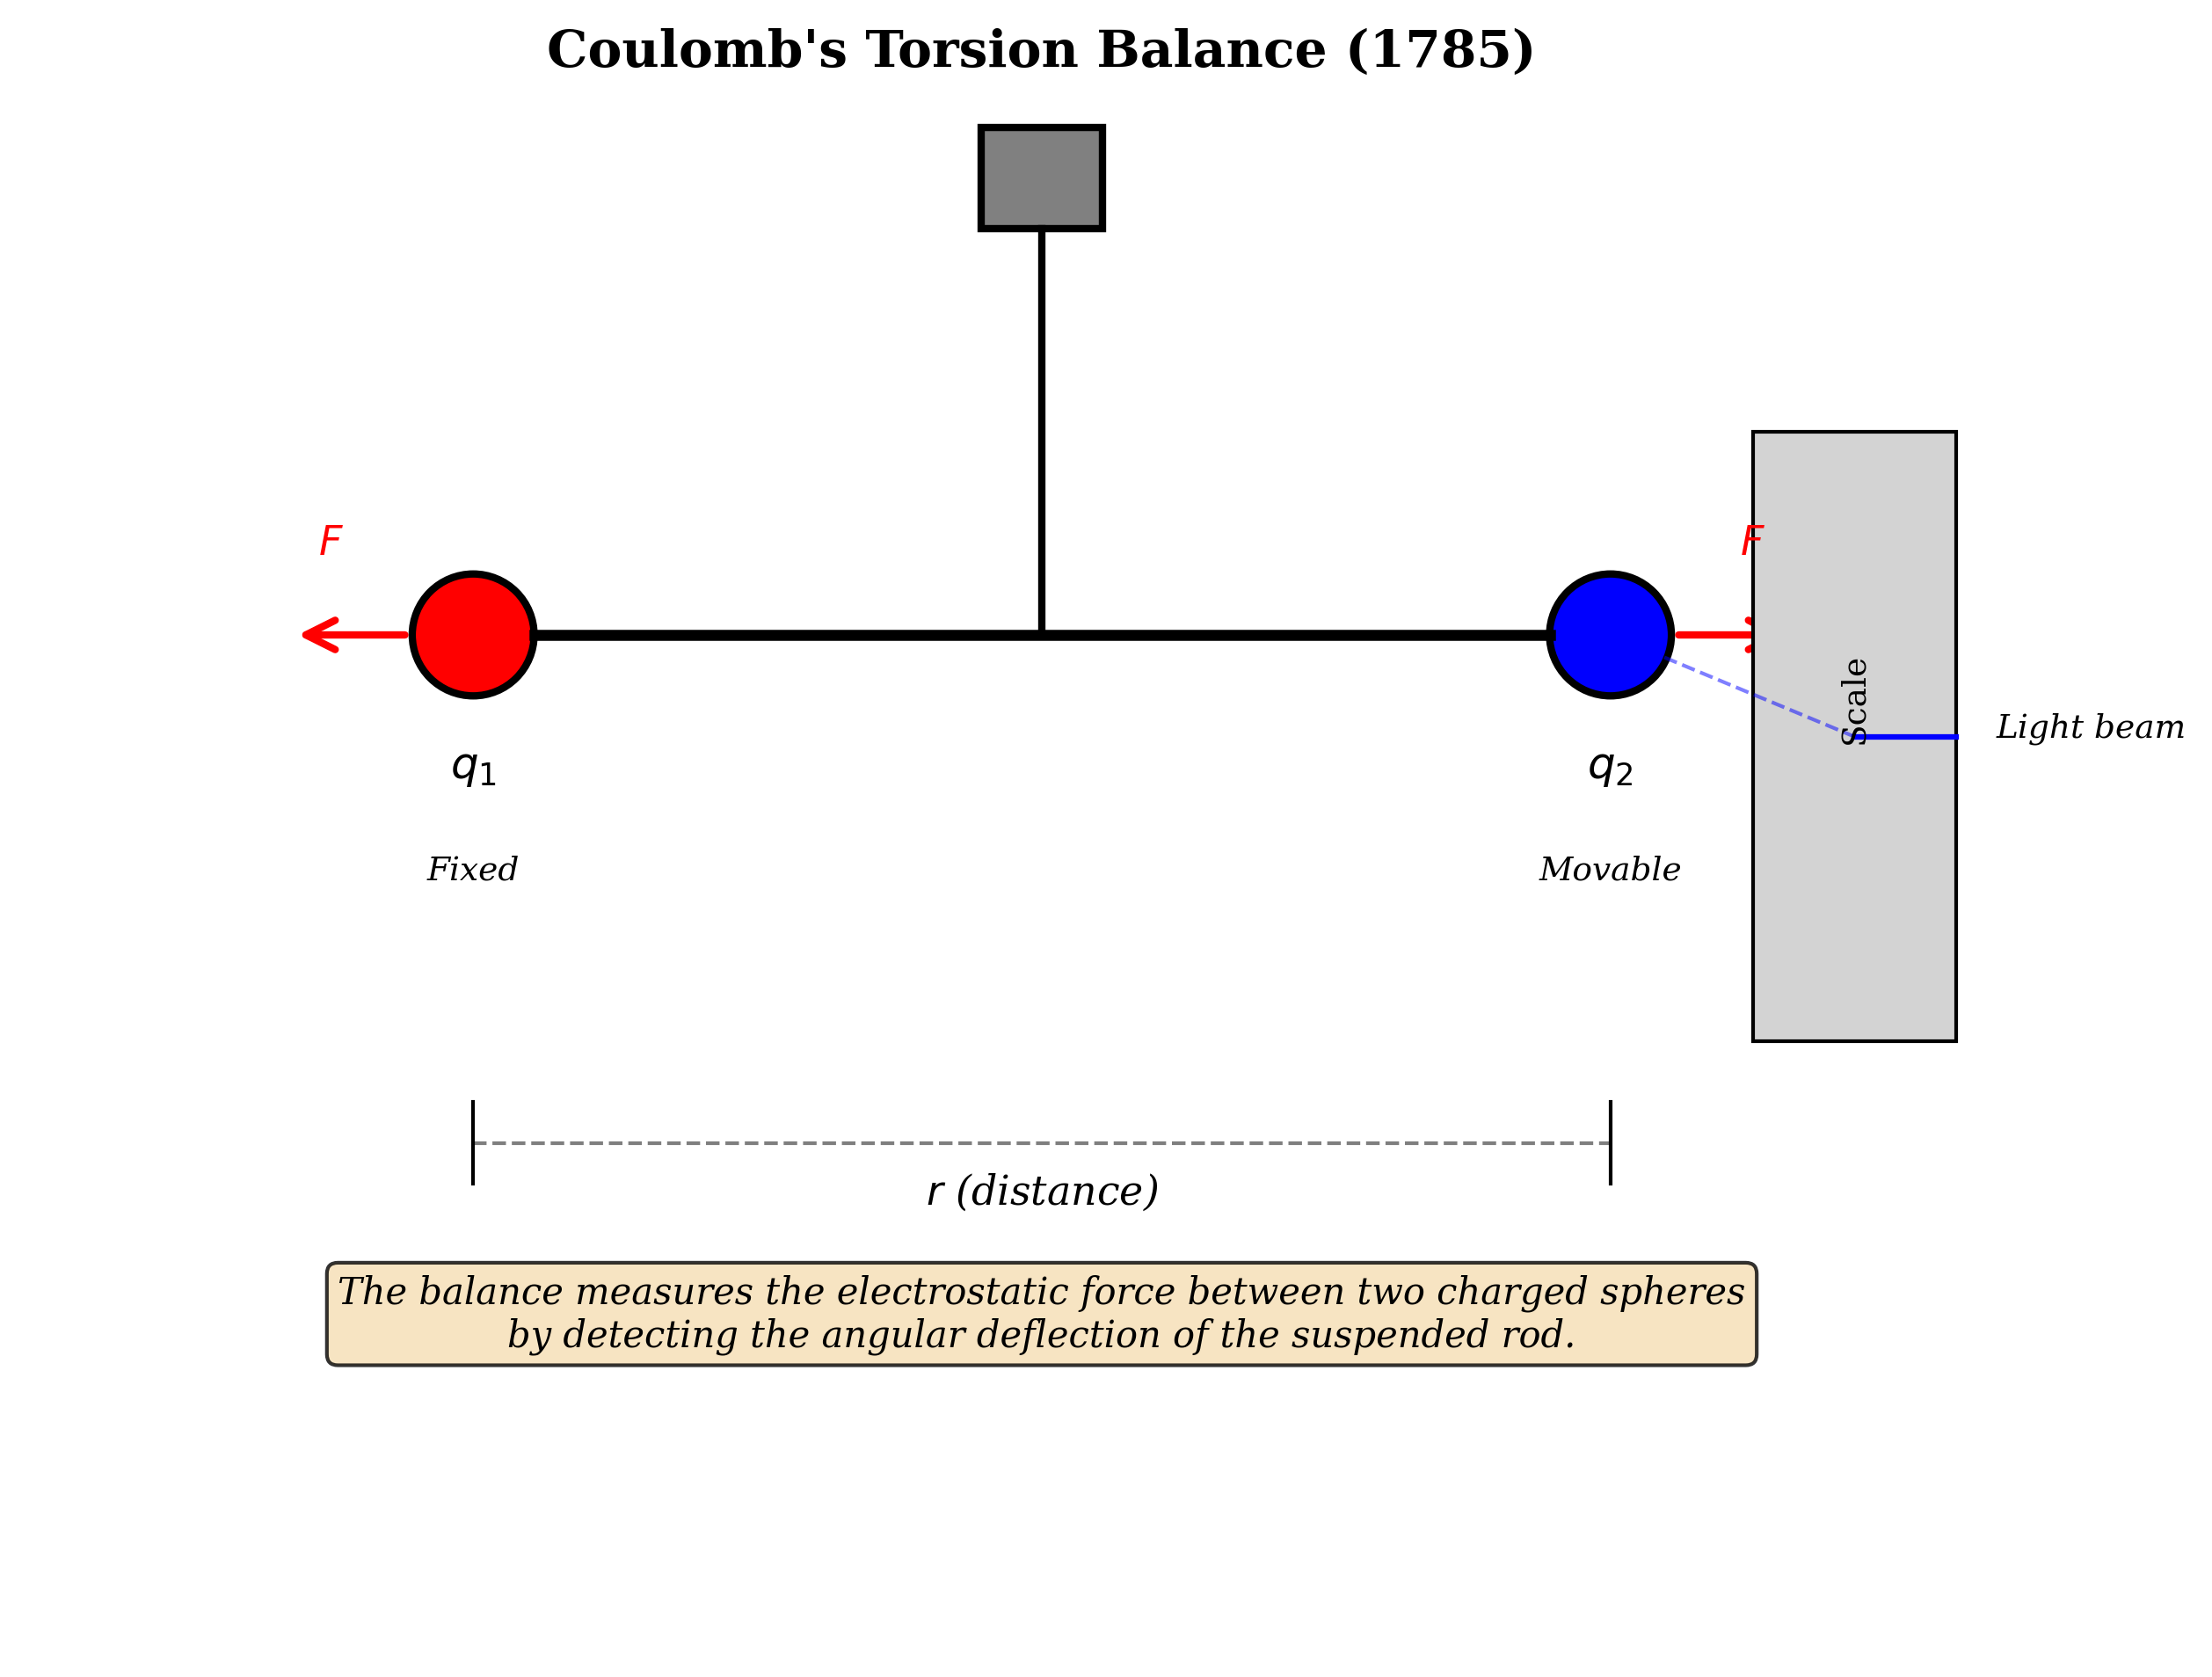
\includegraphics[width=0.7\textwidth]{images/chapter03/coulomb_experiment.png}
\caption{Coulomb's torsion balance experiment (1785). Coulomb used this apparatus to measure the force between charged spheres at different distances, establishing the inverse square law for electrostatic forces. The balance measures the electrostatic force by detecting the angular deflection of the suspended rod when charges are placed at various distances.}
\label{fig:coulomb_experiment}
\end{figure}

Mathematically, Coulomb's law states that the force $\boldsymbol{F}$ between two charges $q_1$ and $q_2$ separated by distance $r$ is:
\begin{equation}
F = k \frac{q_1 q_2}{r^2} \label{eq:coulomb_force}
\end{equation}
where $k = 1/(4\pi\epsilon_0)$ is Coulomb's constant. The force is attractive if the charges have opposite signs and repulsive if they have the same sign.

\begin{figure}[htbp]
\centering
\begin{minipage}{0.48\textwidth}
\centering
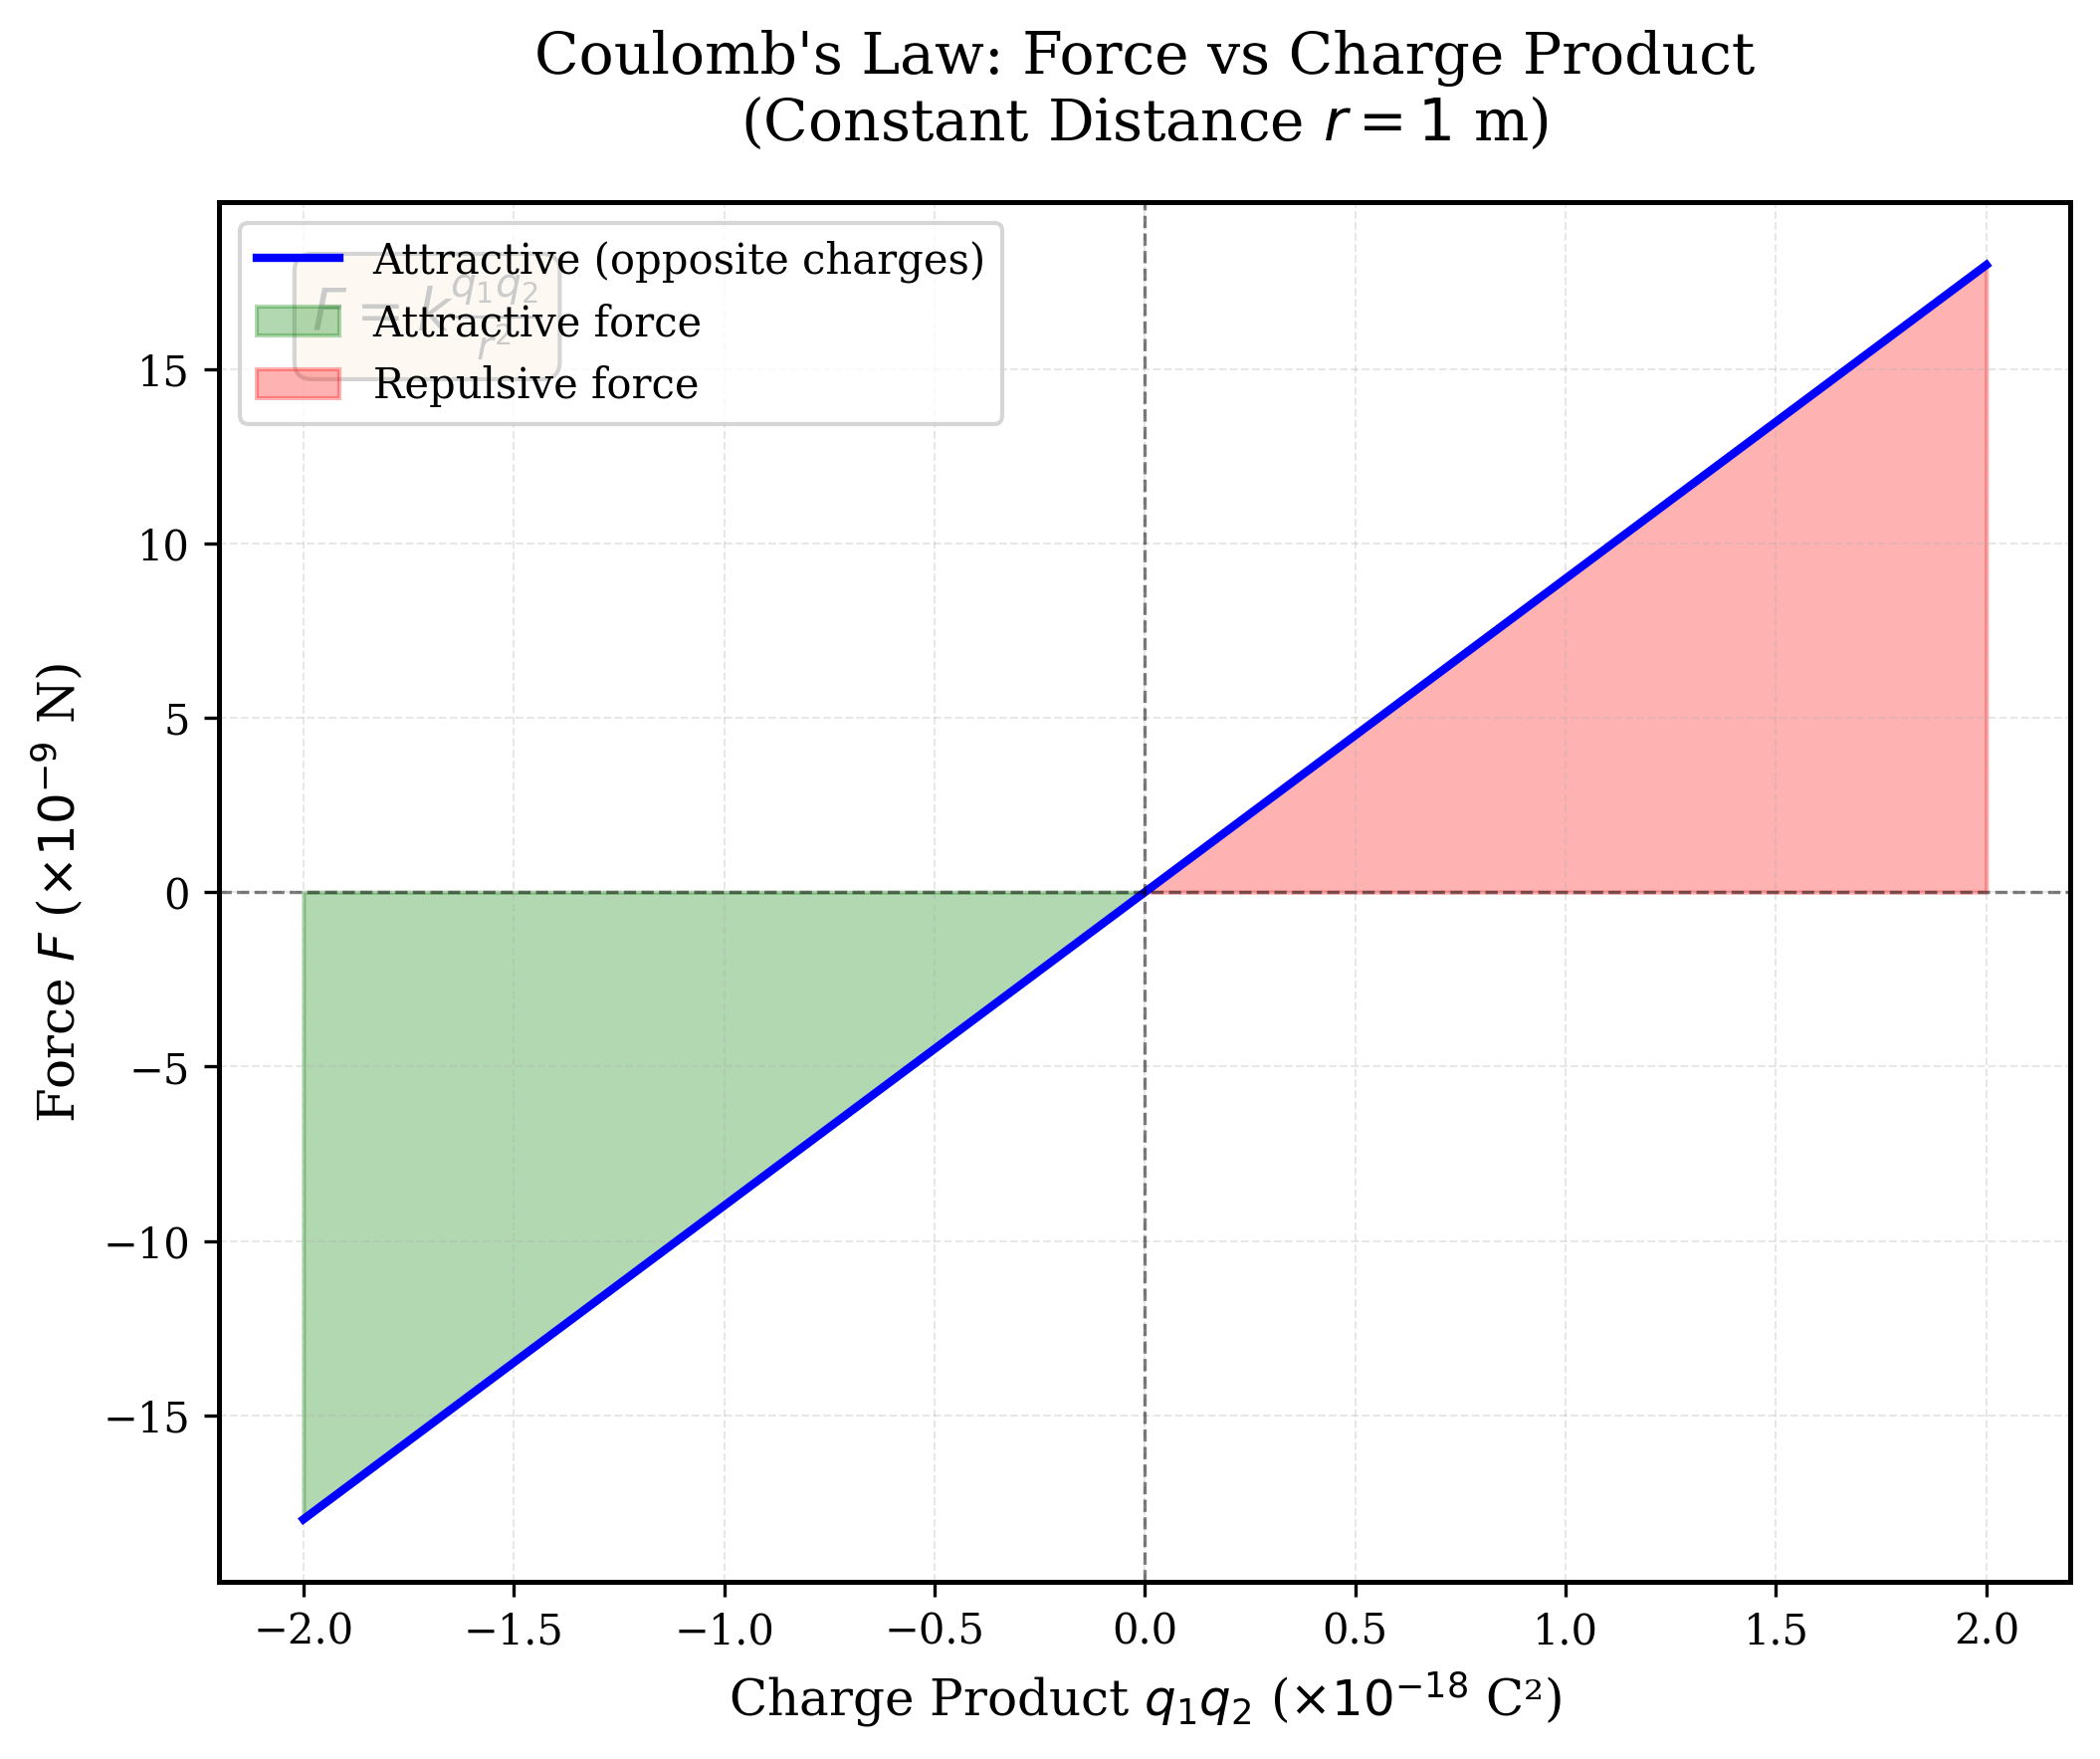
\includegraphics[width=\textwidth]{images/chapter03/coulomb_force_vs_charge.png}
\caption{Force vs charge product at constant distance ($r = 1$ m). The linear relationship shows that force is directly proportional to the product $q_1 q_2$. Negative values indicate attractive forces (opposite charges), positive values indicate repulsive forces (like charges).}
\label{fig:coulomb_force_vs_charge}
\end{minipage}
\hfill
\begin{minipage}{0.48\textwidth}
\centering
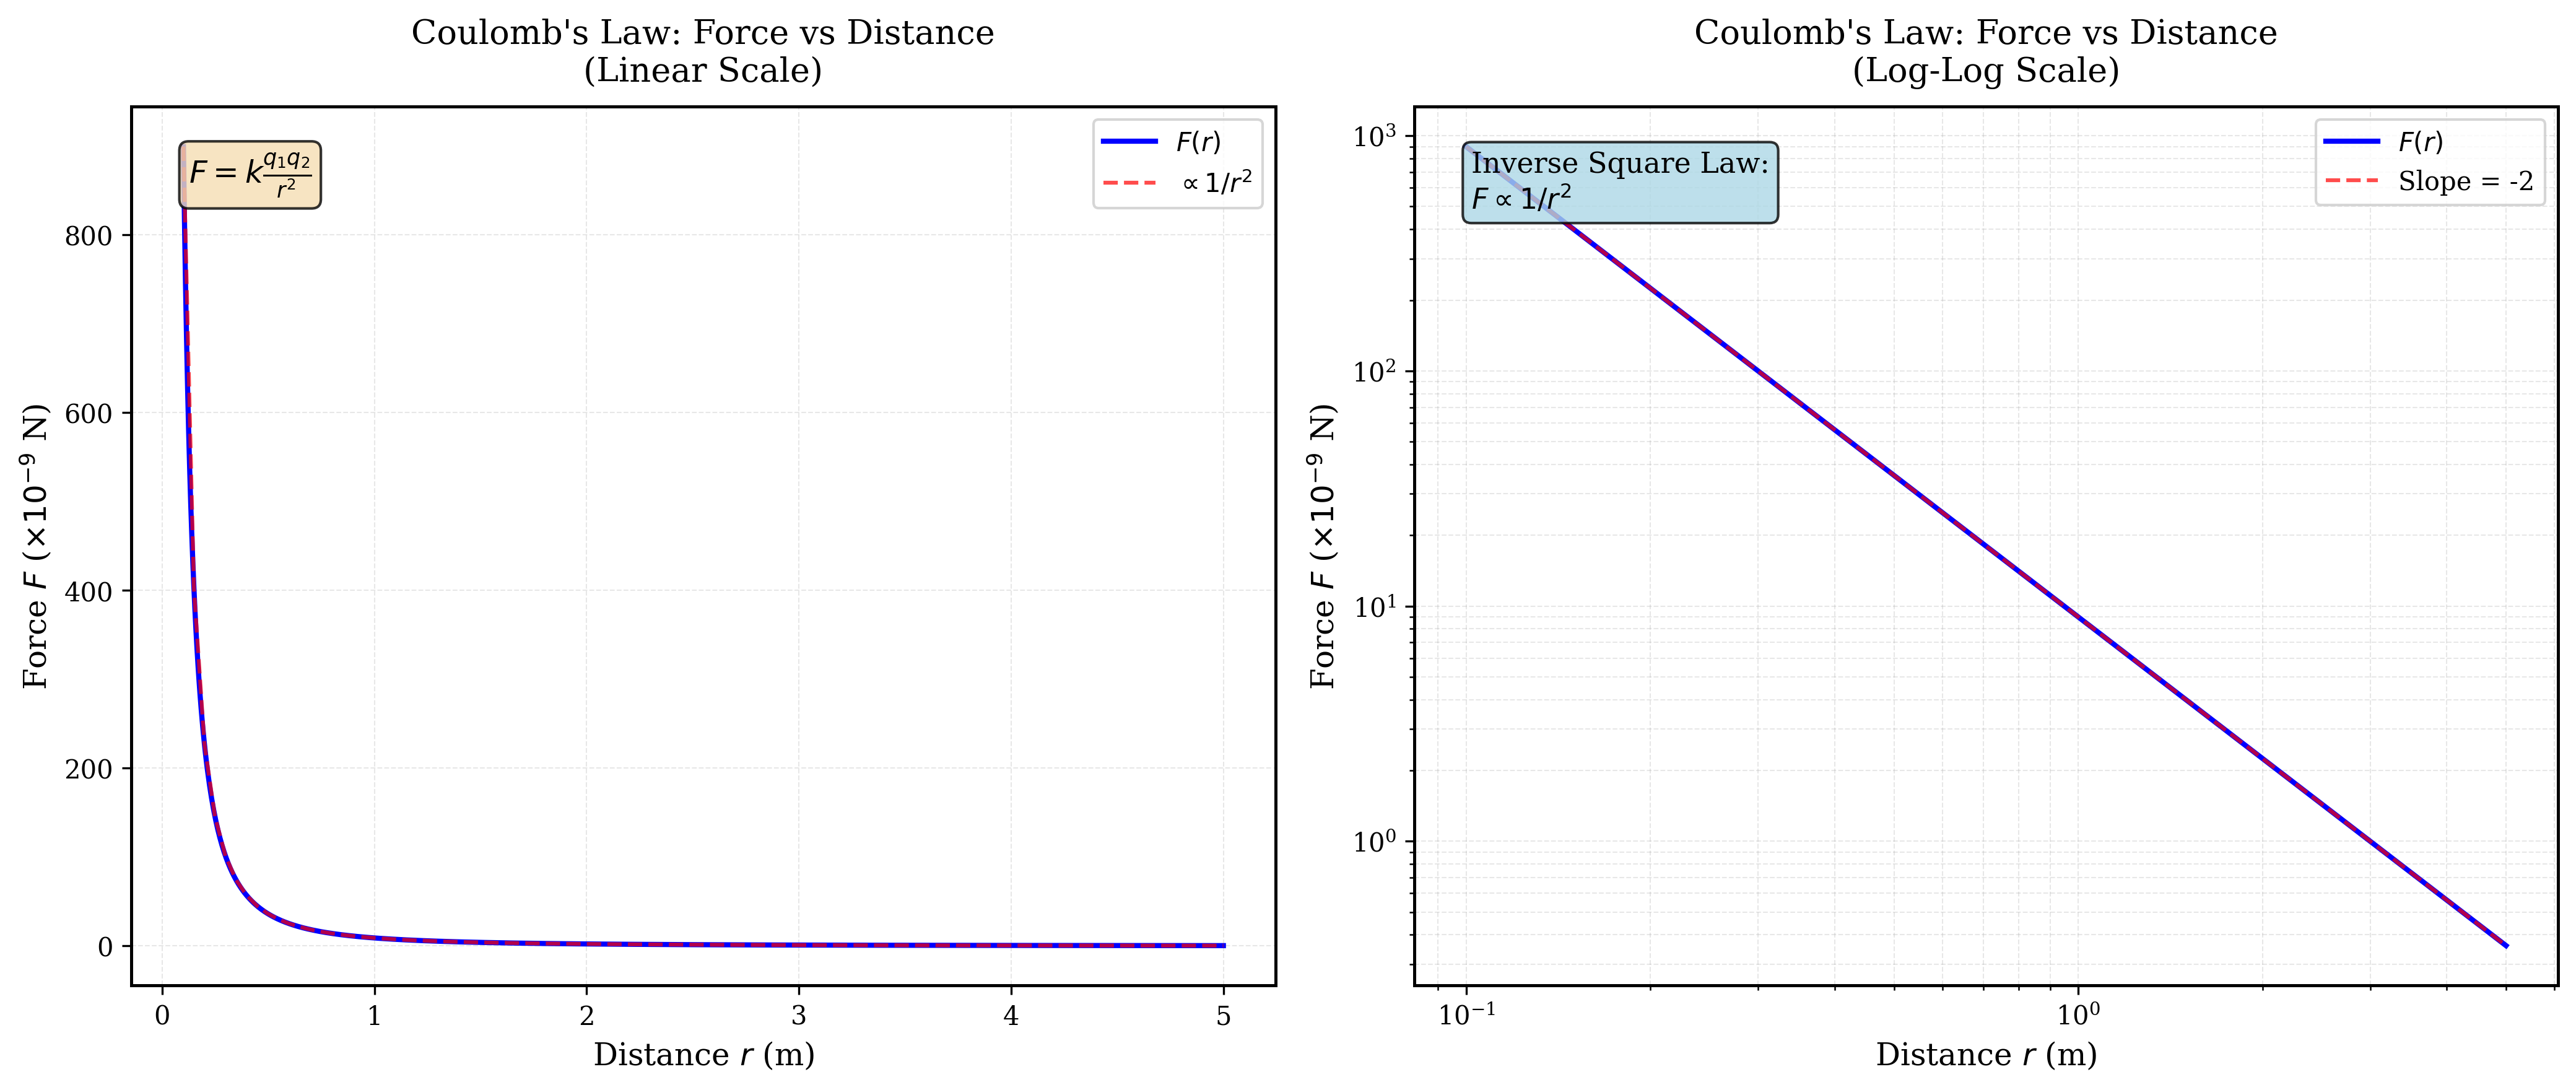
\includegraphics[width=\textwidth]{images/chapter03/coulomb_force_vs_distance.png}
\caption{Force vs distance at constant charge product. Left: Linear scale showing the rapid decrease of force with distance. Right: Log-log scale revealing the inverse square relationship ($F \propto 1/r^2$), evident from the straight line with slope $-2$.}
\label{fig:coulomb_force_vs_distance}
\end{minipage}
\end{figure}

These plots illustrate the fundamental relationships in equation \eqref{eq:coulomb_force}: the force is directly proportional to the charge product and inversely proportional to the square of the distance. The inverse square law is a hallmark of field theories and appears in both electrostatics and gravitation.

This law is remarkably similar to Newton's law of universal gravitation, suggesting a deep parallel between electrical and gravitational forces. Coulomb's law implies that electric charges create electric fields in the space around them. The electric field $\boldsymbol{E}$ at a point due to a charge $q$ is:
\begin{equation}
\boldsymbol{E} = \frac{1}{4\pi\epsilon_0} \frac{q}{r^2} \hat{\boldsymbol{r}} \label{eq:coulomb_field}
\end{equation}
where $\hat{\boldsymbol{r}}$ is the unit vector pointing from the charge to the observation point.

\begin{figure}[htbp]
\centering
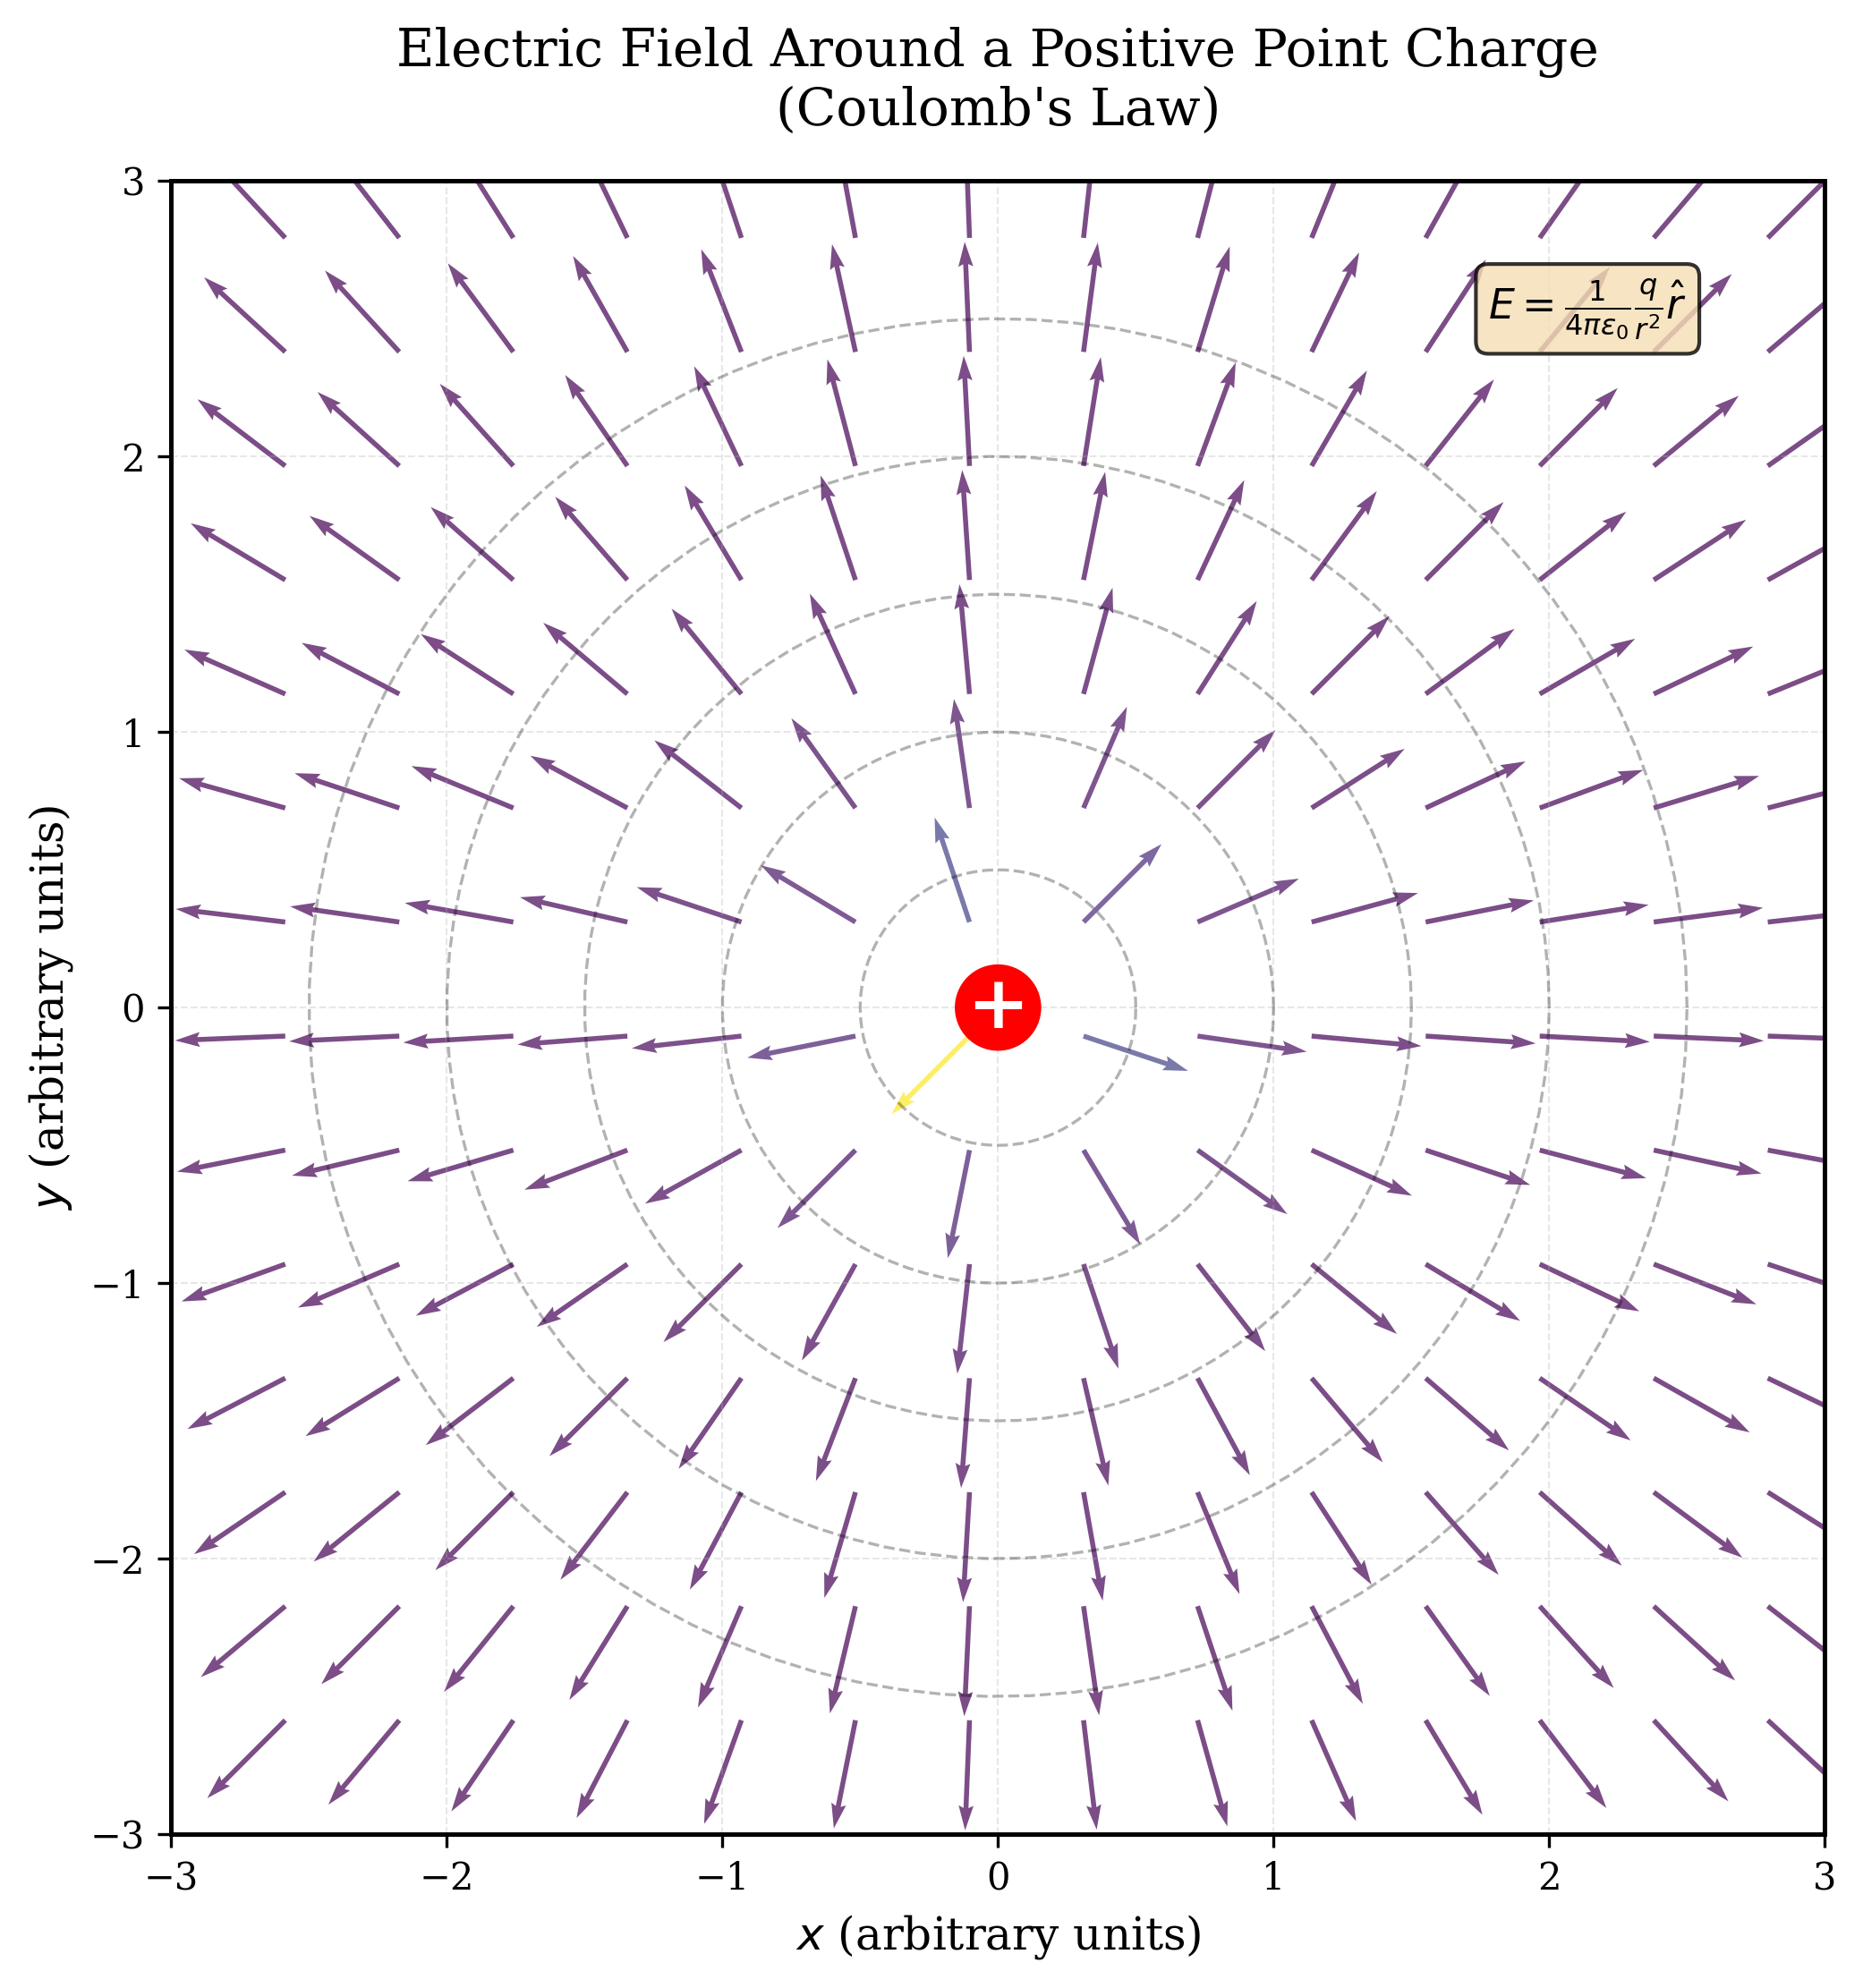
\includegraphics[width=0.7\textwidth]{images/chapter03/coulomb_law_field.png}
\caption{Electric field around a positive point charge, illustrating the field representation of Coulomb's law. The field lines radiate outward from the charge, with the field strength decreasing as $1/r^2$ with distance, as given by equation \eqref{eq:coulomb_field}. The color intensity represents the magnitude of the electric field.}
\label{fig:coulomb_law_field}
\end{figure}

\subsubsection{Ampère's Law (1820)}

In 1820, Hans Christian Ørsted made a revolutionary discovery: an electric current produces a magnetic field. This was the first clear evidence that electricity and magnetism are related. Building on this, André-Marie Ampère formulated a mathematical law describing how electric currents create magnetic fields.

\begin{figure}[htbp]
\centering
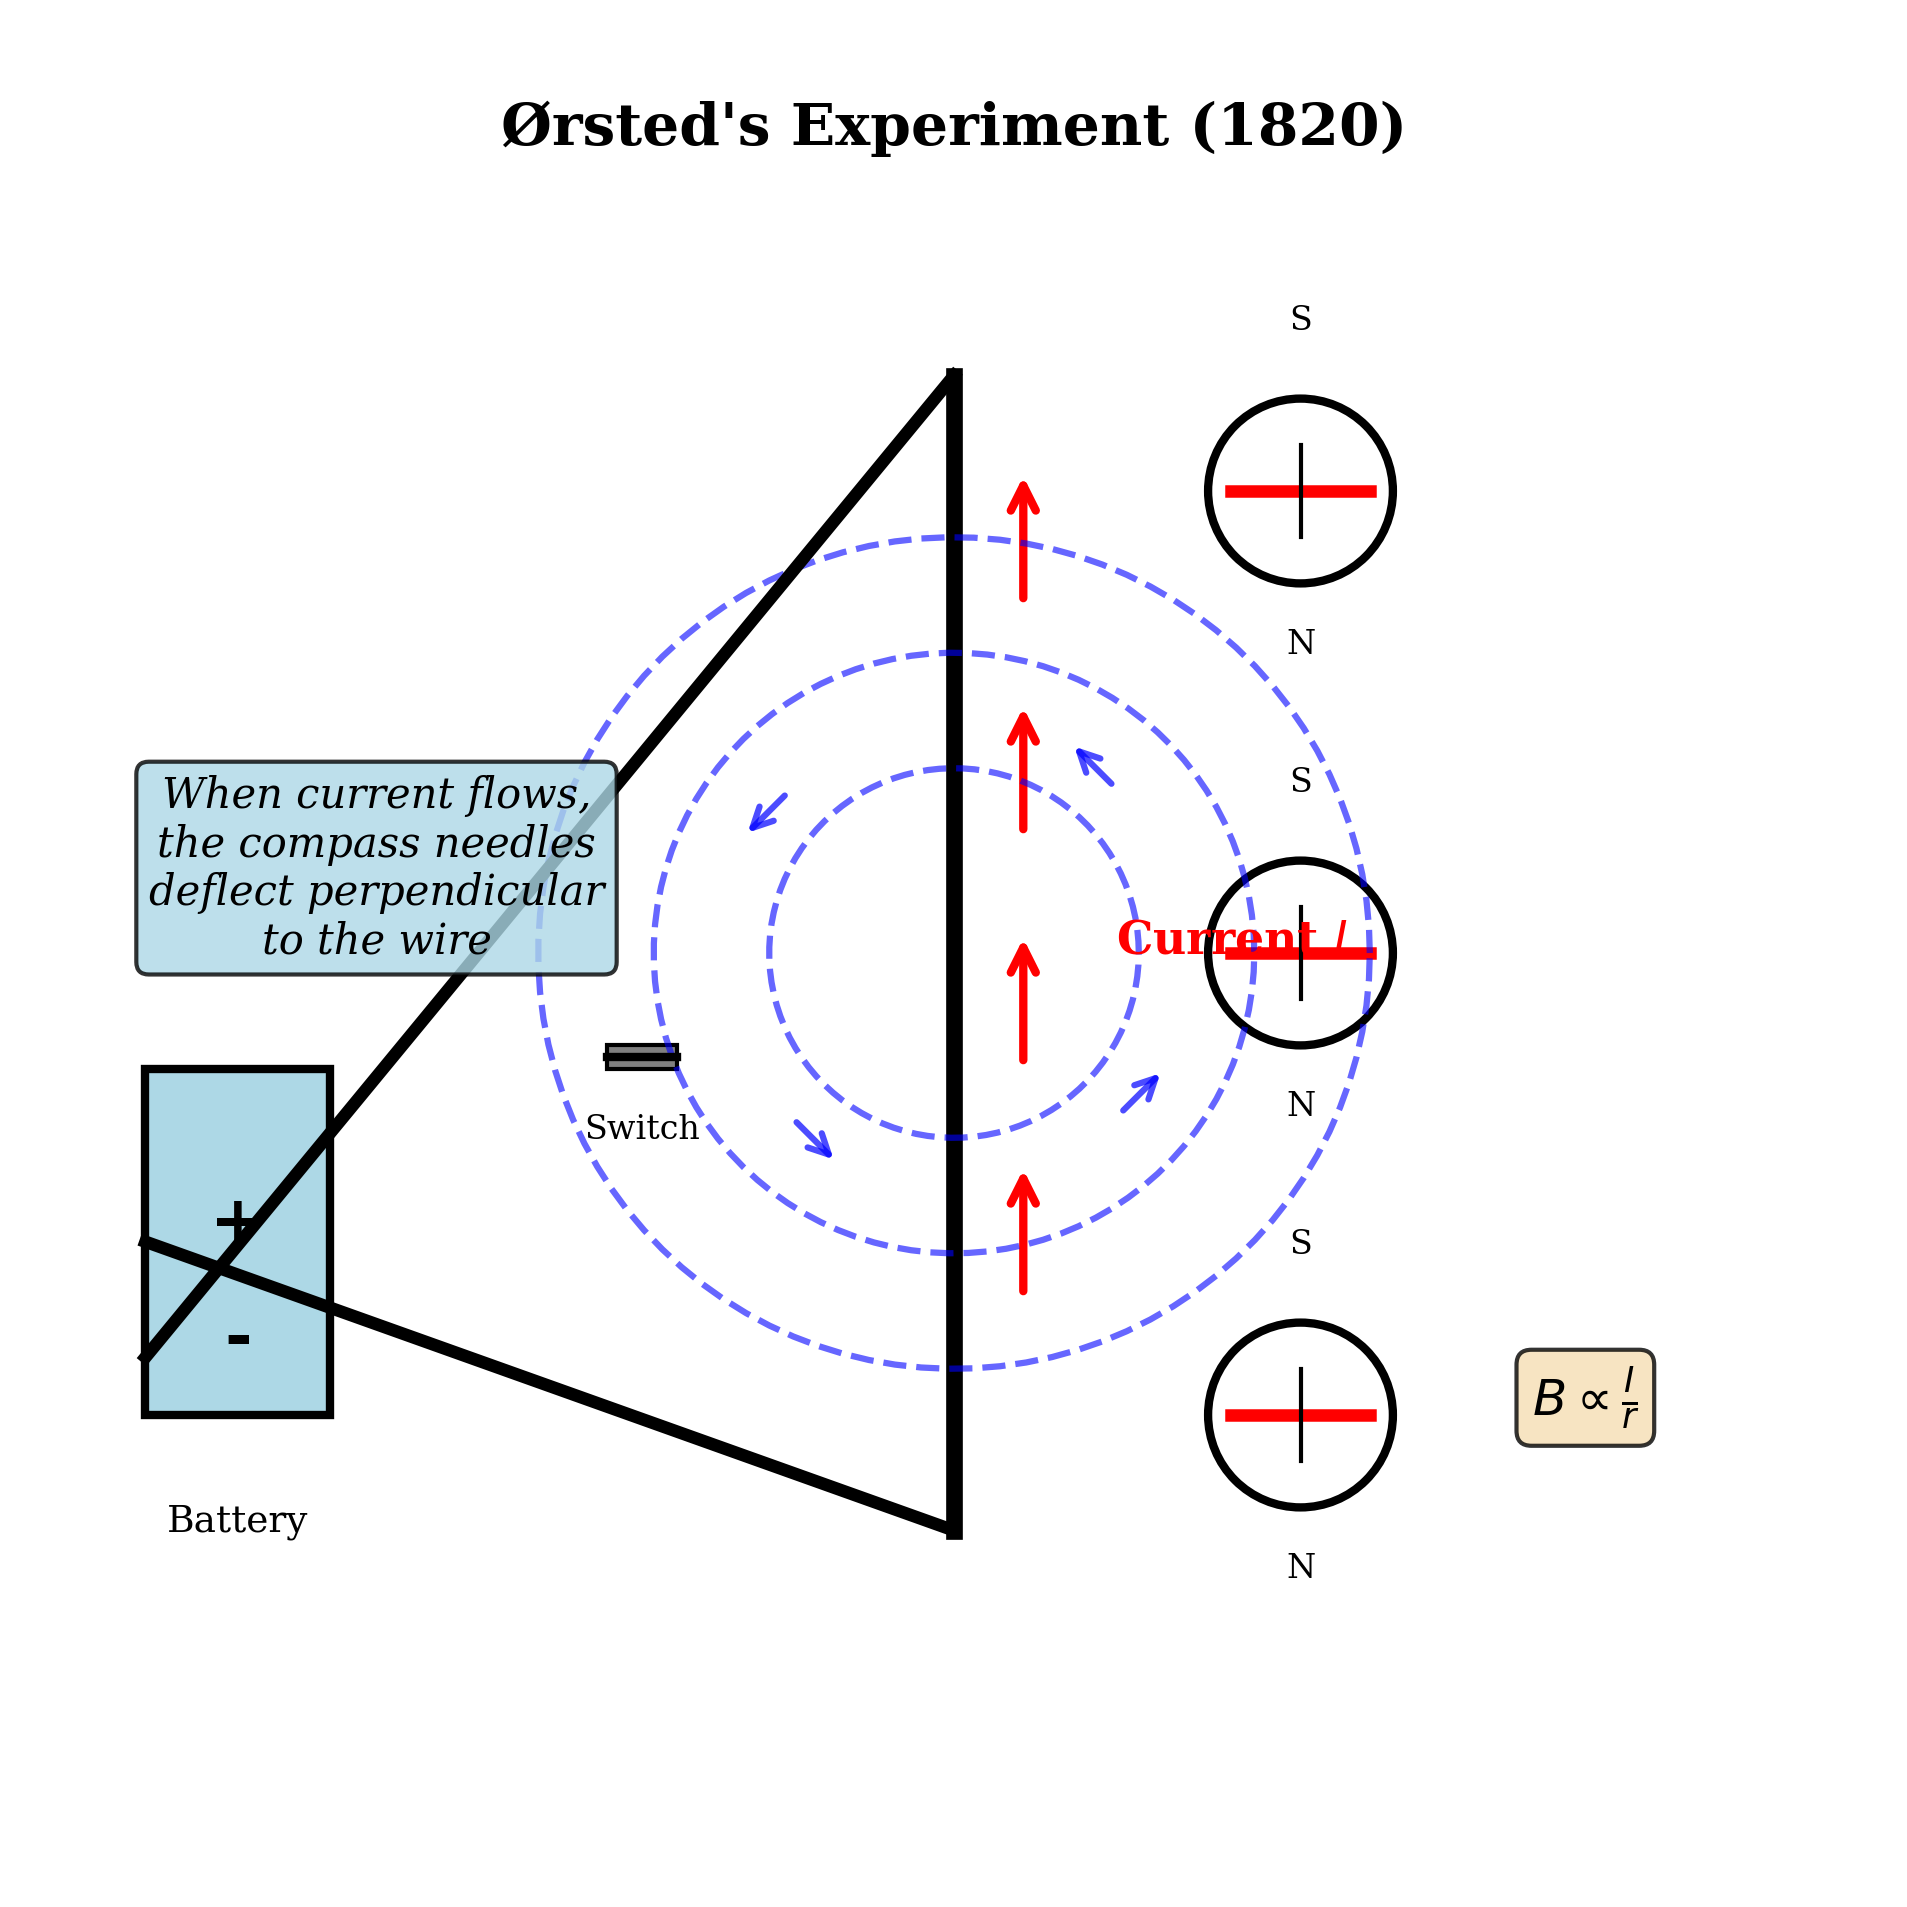
\includegraphics[width=0.7\textwidth]{images/chapter03/ampere_experiment.png}
\caption{Ørsted's experiment (1820) demonstrating that an electric current deflects a compass needle, revealing the connection between electricity and magnetism. When current flows through the vertical wire, the compass needles align perpendicular to the wire, indicating a circular magnetic field around the current. Ampère later quantified this relationship mathematically.}
\label{fig:ampere_experiment}
\end{figure}

Ampère's law states that the magnetic field $\boldsymbol{B}$ circulates around an electric current. For a steady current $I$ flowing through a wire, the magnetic field forms closed loops around the wire. The mathematical expression, in its original form, relates the circulation (line integral) of the magnetic field around a closed loop to the current passing through that loop:
\begin{equation}
\oint \boldsymbol{B} \cdot d\boldsymbol{l} = \mu_0 I \label{eq:ampere_integral}
\end{equation}
where $\mu_0$ is the permeability of free space and $I$ is the current enclosed by the loop.

In differential form, this becomes:
\begin{equation}
\nabla \times \boldsymbol{B} = \mu_0 \boldsymbol{J} \label{eq:ampere_differential}
\end{equation}
where $\boldsymbol{J}$ is the current density. This law successfully explained how electric currents create magnetic fields, but it had a limitation: it only worked for steady (constant) currents. When currents changed with time, the law became inconsistent, as we shall see.

\begin{figure}[htbp]
\centering
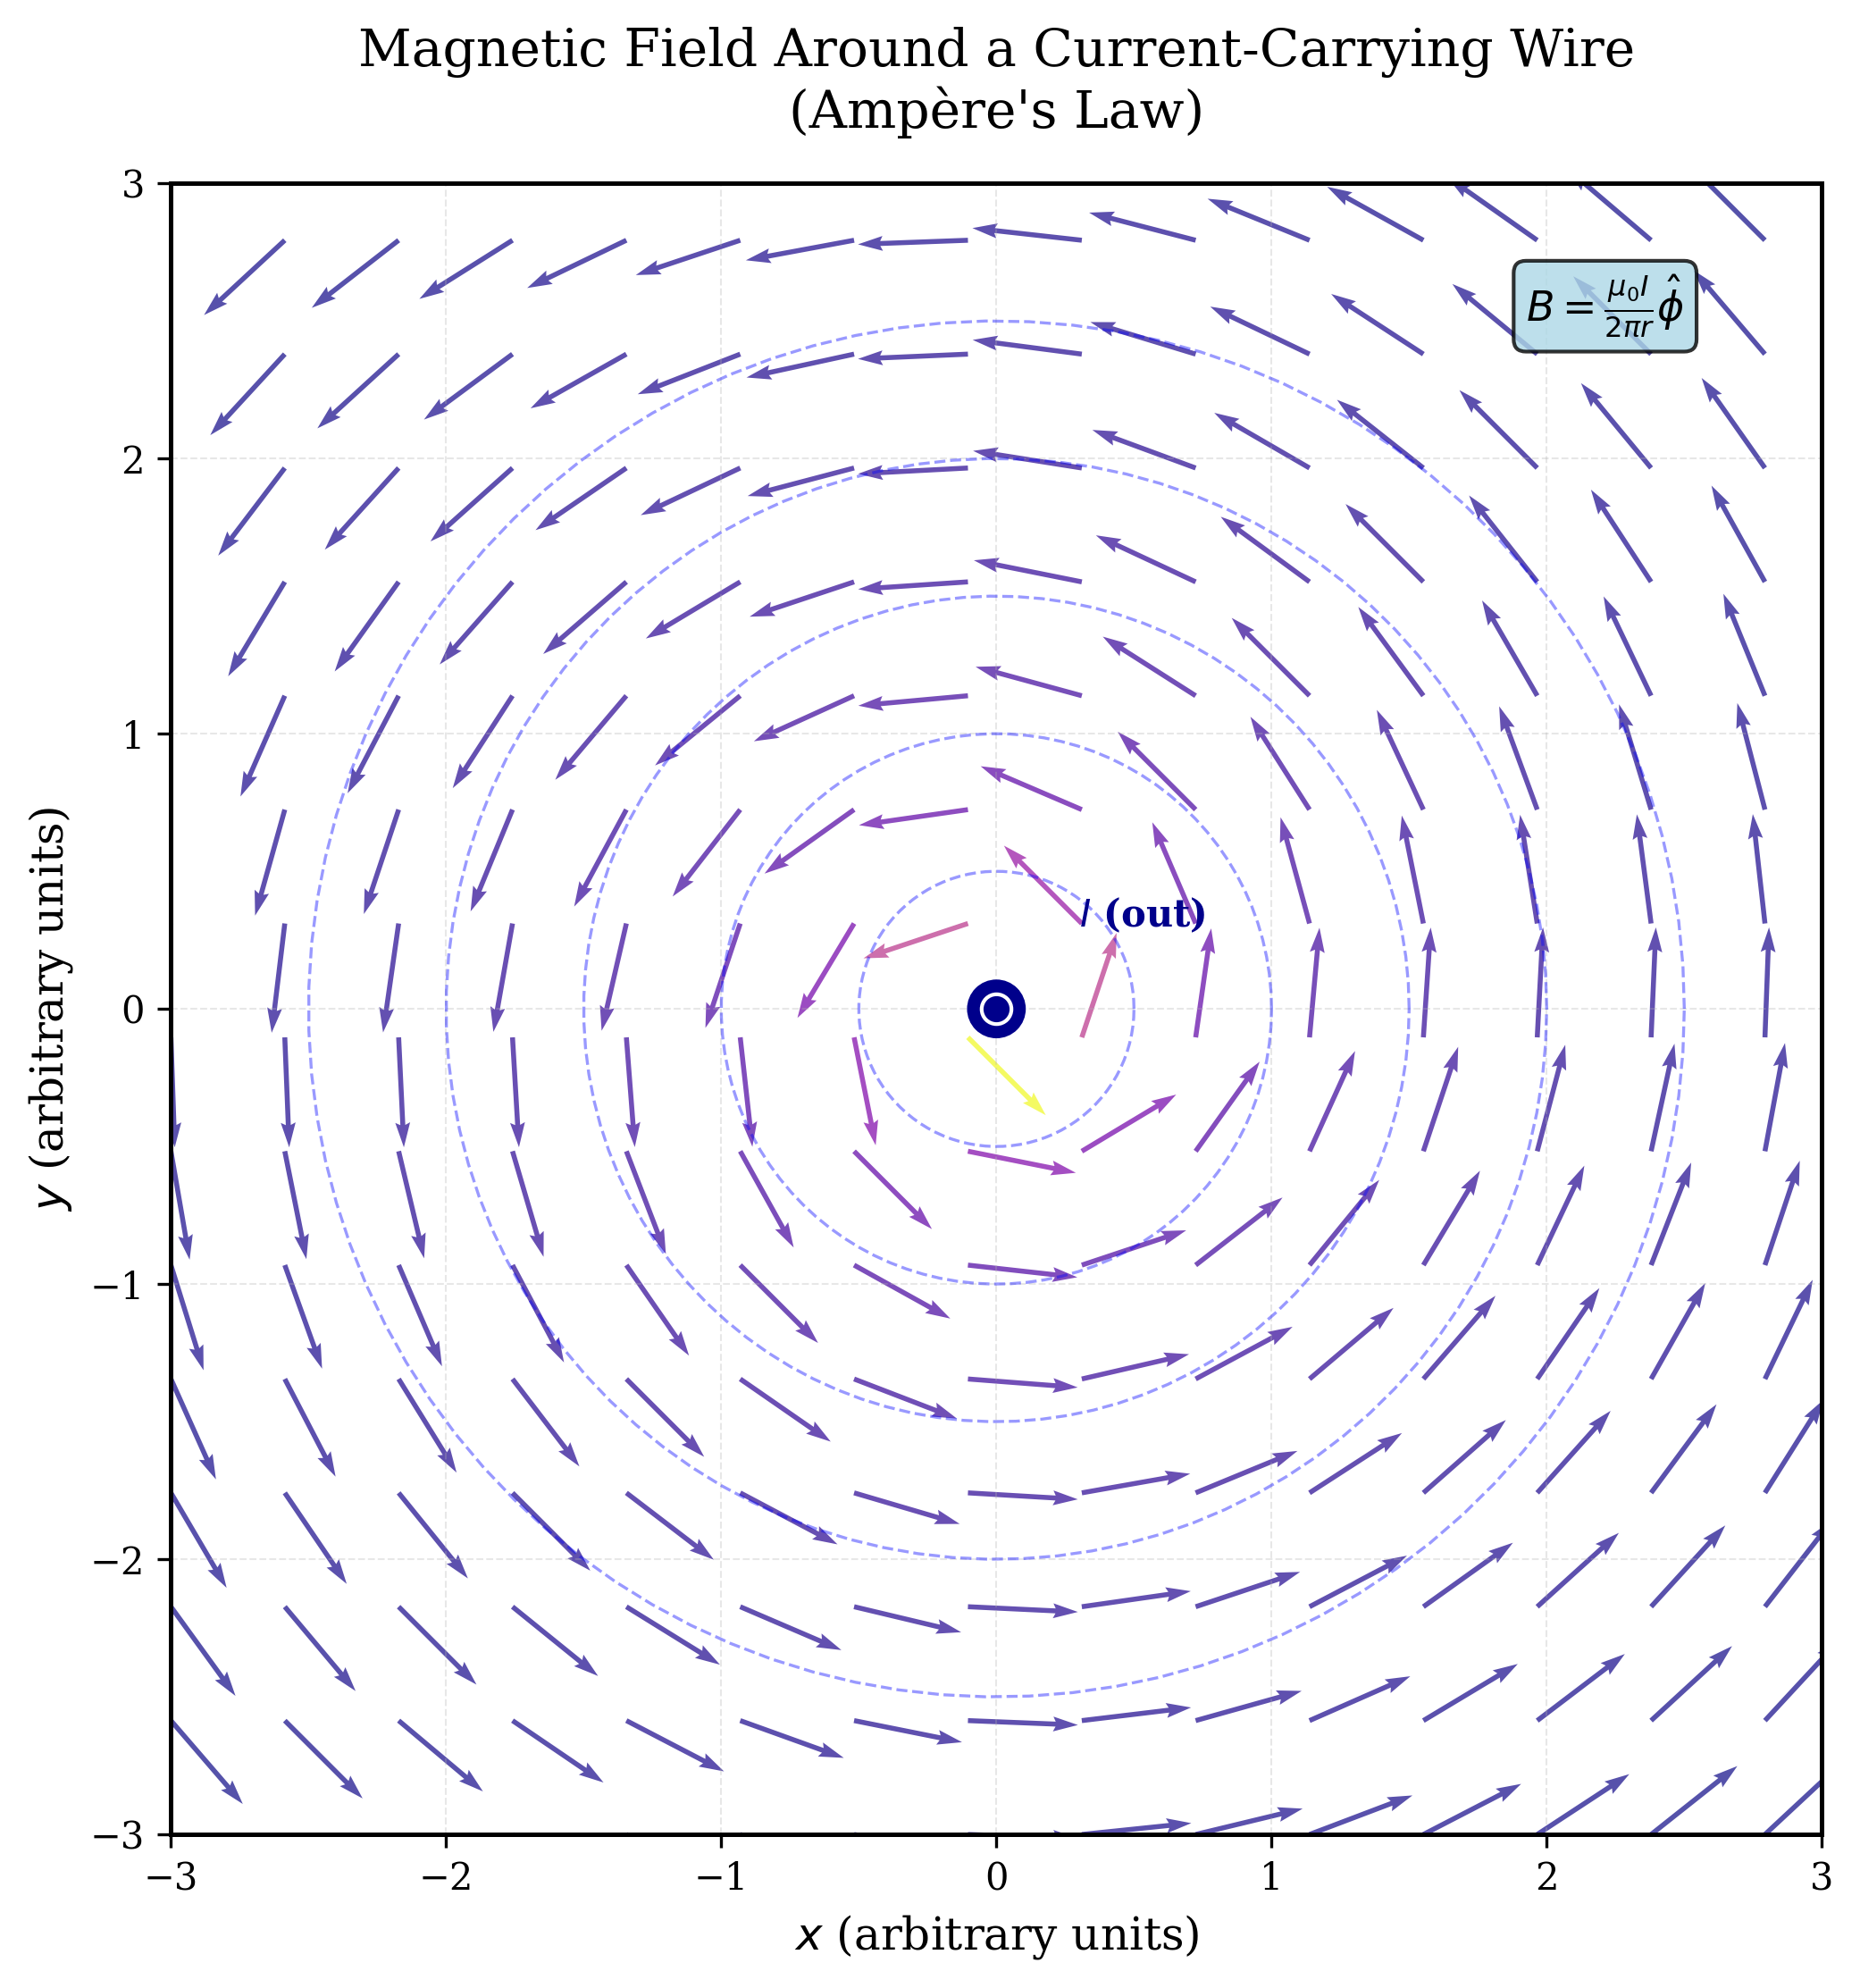
\includegraphics[width=0.7\textwidth]{images/chapter03/ampere_law_field.png}
\caption{Magnetic field around a current-carrying wire, illustrating Ampère's law (equations \eqref{eq:ampere_integral} and \eqref{eq:ampere_differential}). The magnetic field forms circular loops around the wire, with the field strength decreasing as $1/r$ with distance from the wire. The dot at the center indicates current flowing out of the page.}
\label{fig:ampere_law_field}
\end{figure}

\subsubsection{Faraday's Law of Induction (1831)}

In 1831, Michael Faraday made one of the most important discoveries in the history of physics: a changing magnetic field creates an electric field. This phenomenon, called electromagnetic induction, is the principle behind electric generators and transformers.

\begin{figure}[htbp]
\centering
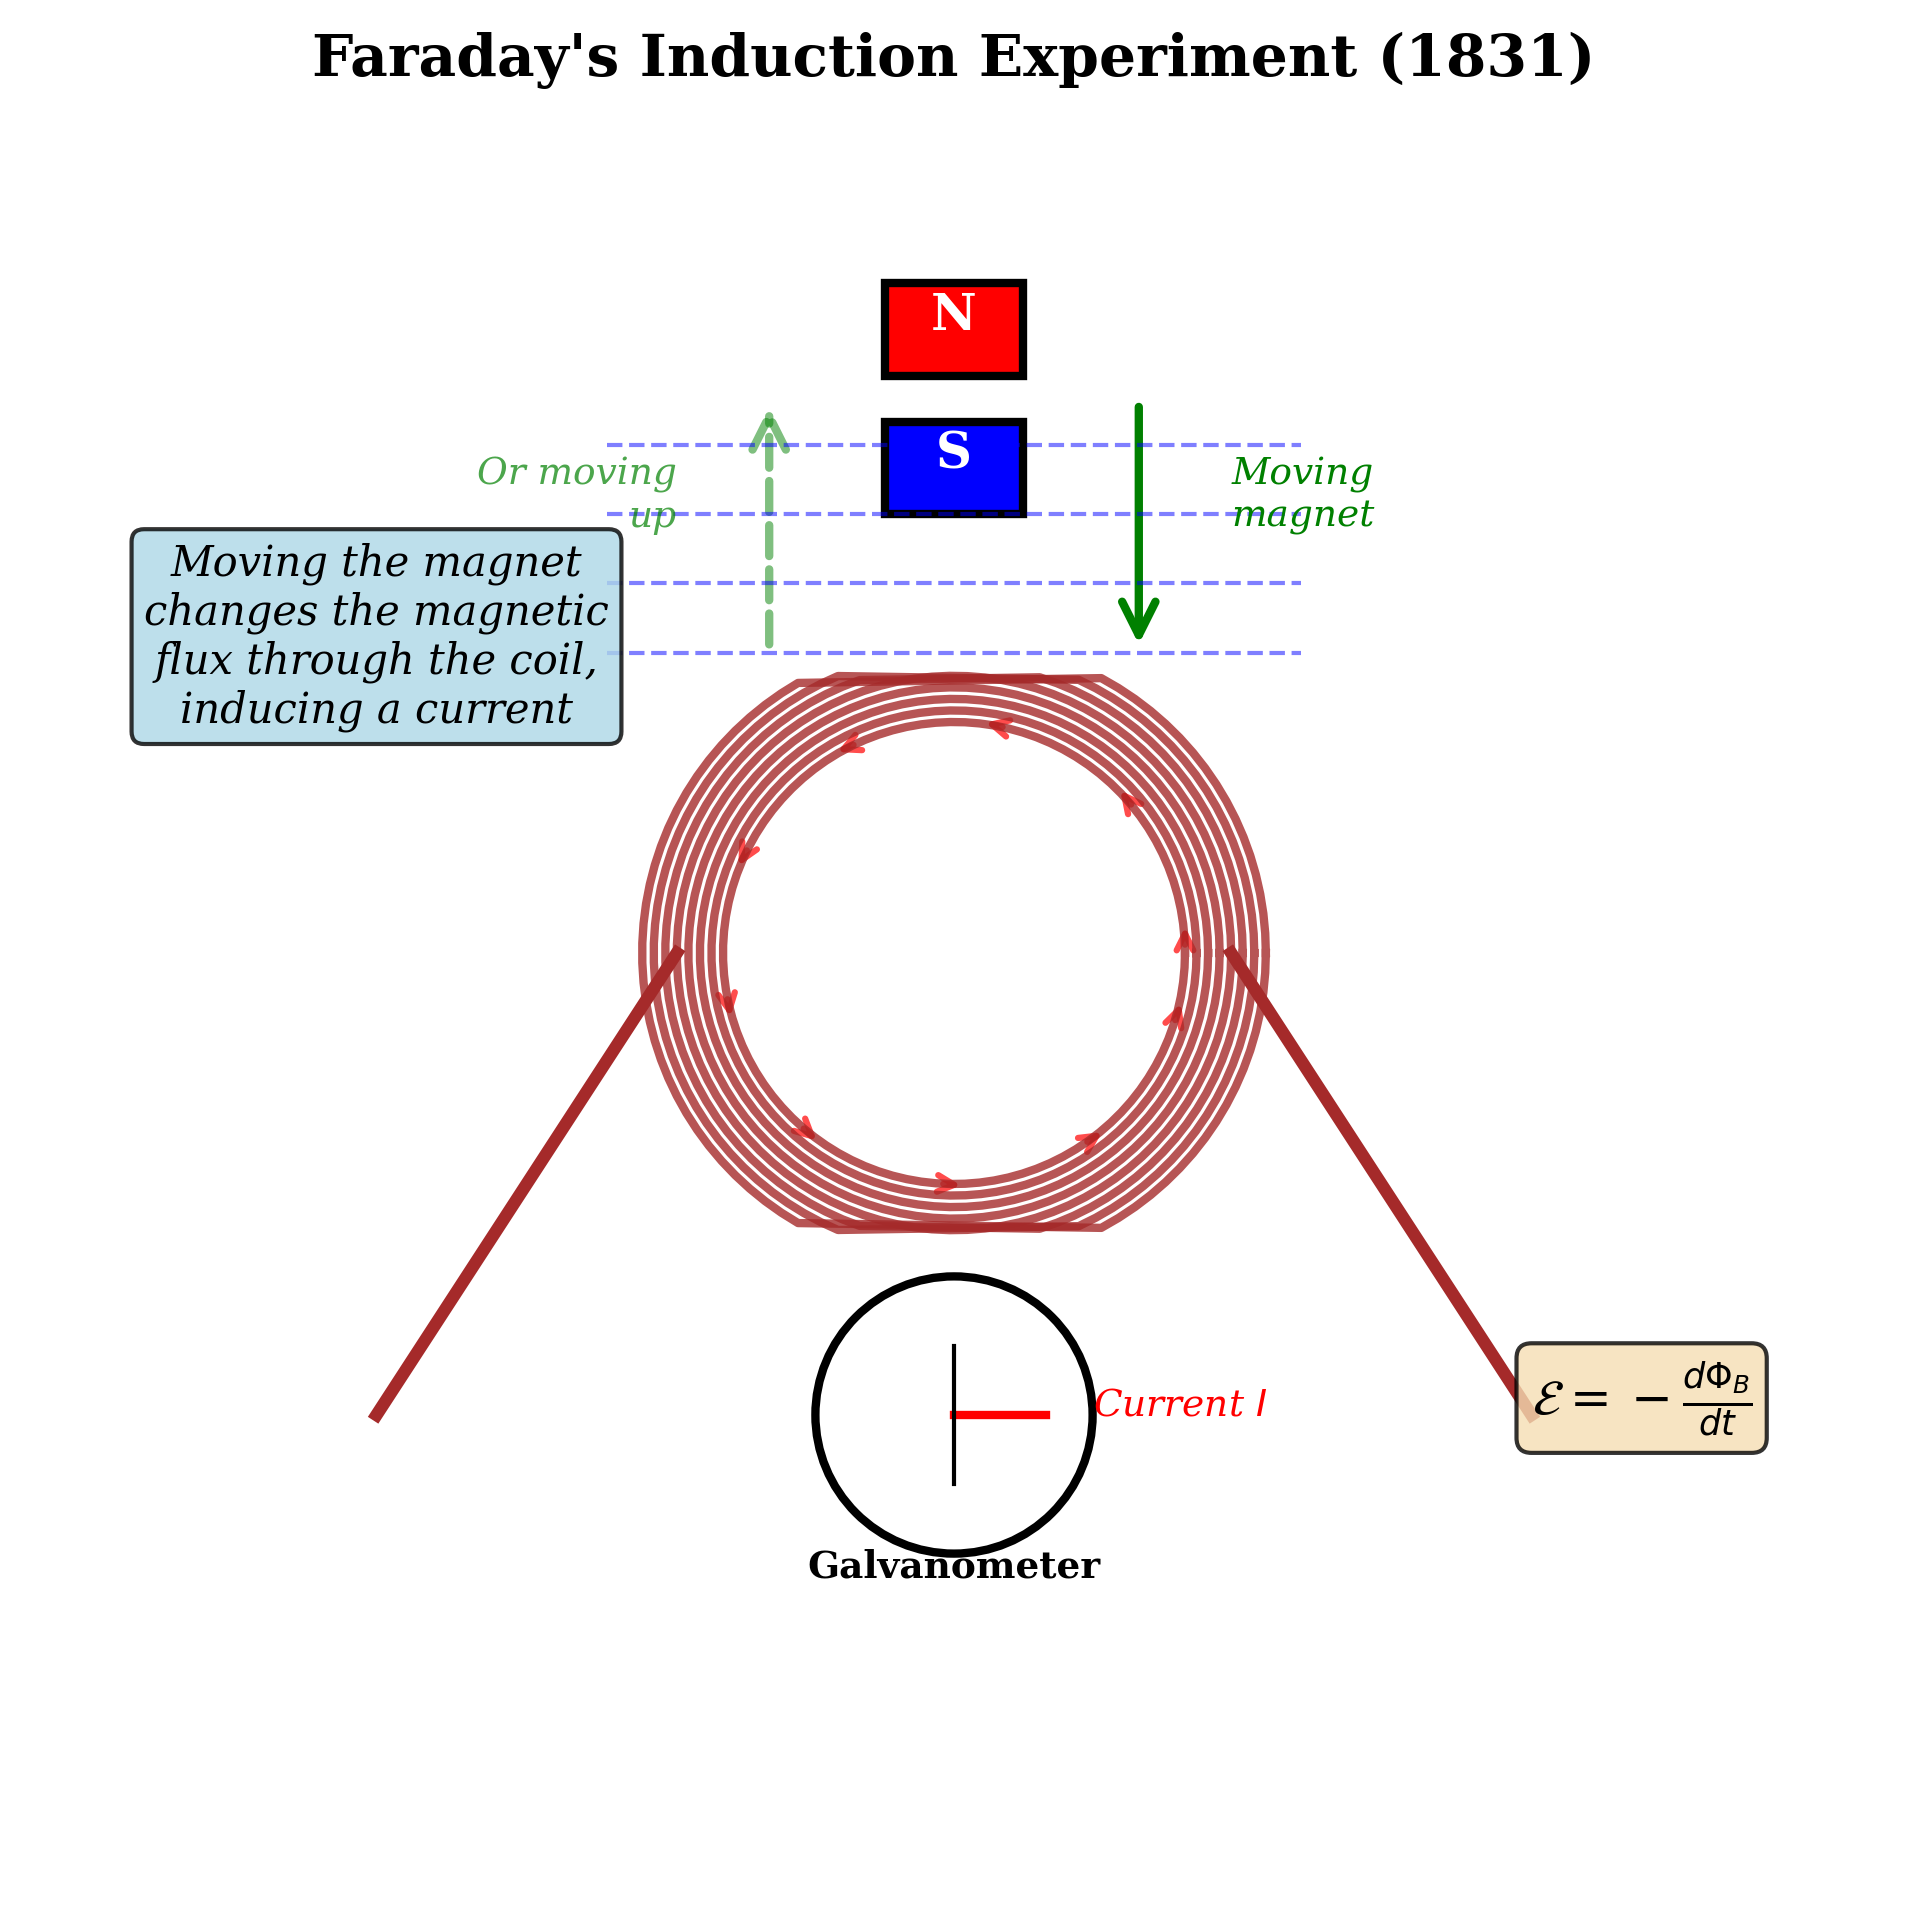
\includegraphics[width=0.7\textwidth]{images/chapter03/faraday_experiment.png}
\caption{Faraday's induction experiment (1831). When a magnet is moved near a coil of wire, or when the magnetic field through a loop changes, an electric current is induced in the coil, detected by the galvanometer. The direction of the induced current opposes the change in magnetic flux (Lenz's law). This discovery established the fundamental relationship between changing magnetic fields and electric currents.}
\label{fig:faraday_experiment}
\end{figure}

Faraday's experiments showed that when a magnet moves near a coil of wire, or when the magnetic field through a loop changes, an electric current is induced in the loop. The key insight is that it is not the magnetic field itself, but its \emph{change} that matters. The faster the magnetic field changes, the stronger the induced electric field.

The mathematical expression of Faraday's law relates the rate of change of magnetic flux through a surface to the electric field induced around the boundary of that surface:
\begin{equation}
\oint \boldsymbol{E} \cdot d\boldsymbol{l} = -\frac{d\Phi_B}{dt} \label{eq:faraday_integral}
\end{equation}
where $\Phi_B$ is the magnetic flux through the surface. The negative sign indicates that the induced electric field opposes the change in magnetic field (Lenz's law).

In differential form, Faraday's law becomes:
\begin{equation}
\nabla \times \boldsymbol{E} = -\frac{\partial \boldsymbol{B}}{\partial t} \label{eq:faraday_differential}
\end{equation}
This equation shows that a changing magnetic field creates a circulating (curl) electric field. This was a profound discovery because it revealed a deep symmetry: just as currents create magnetic fields, changing magnetic fields create electric fields.

\begin{figure}[htbp]
\centering
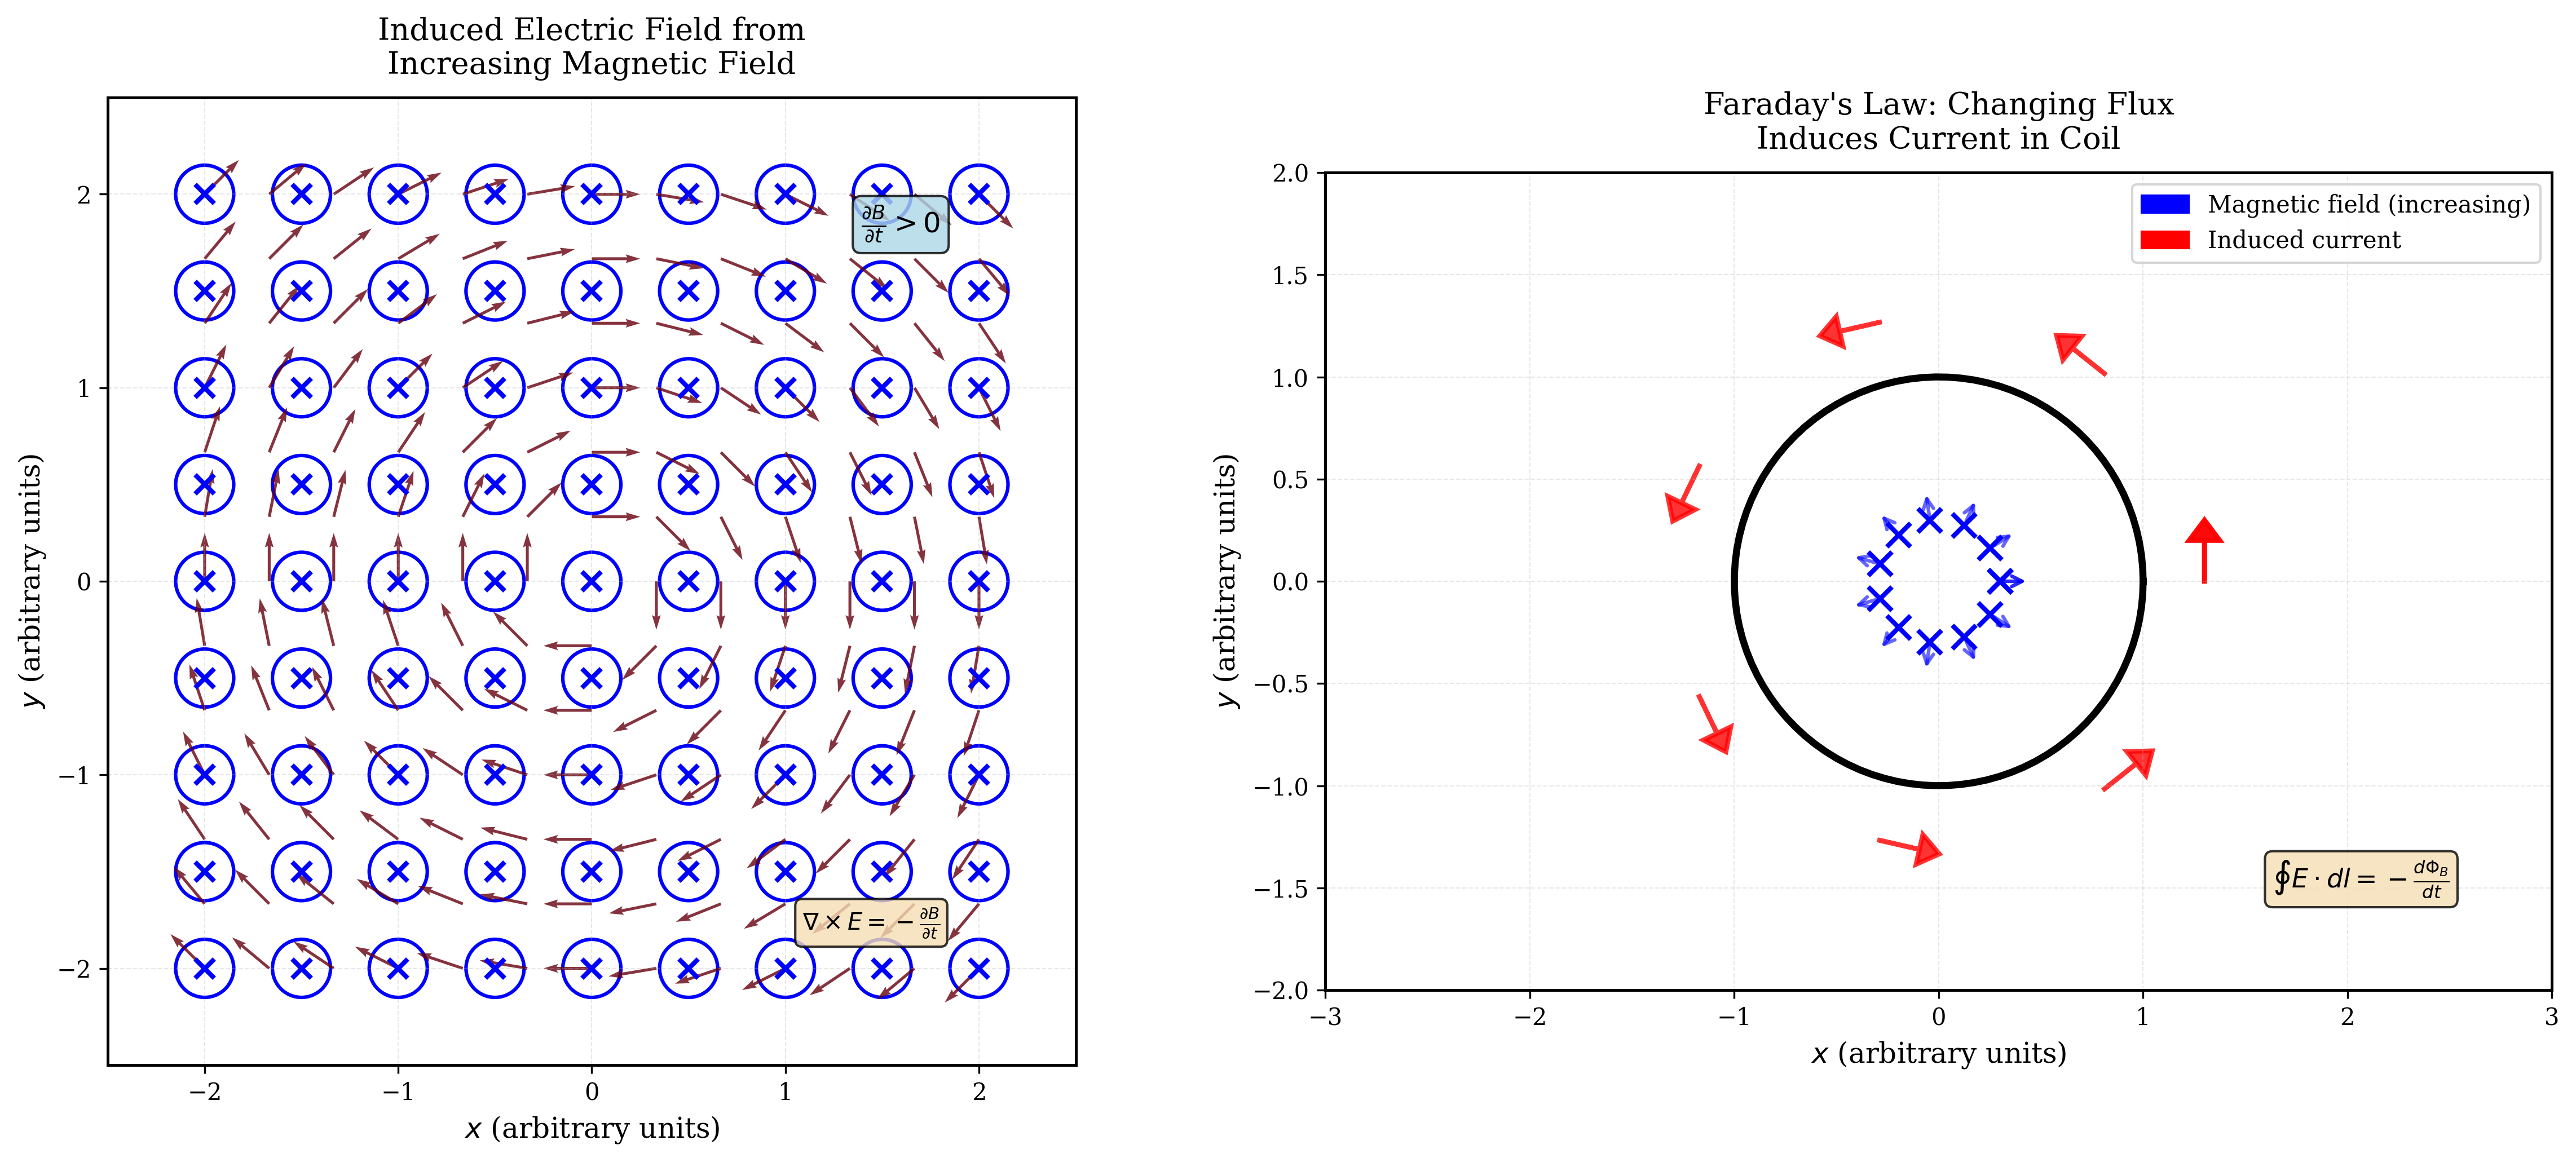
\includegraphics[width=0.9\textwidth]{images/chapter03/faraday_law_induction.png}
\caption{Faraday's law of electromagnetic induction (equations \eqref{eq:faraday_integral} and \eqref{eq:faraday_differential}). Left panel: A uniform magnetic field increasing into the page (indicated by X symbols) induces a circular electric field. Right panel: A changing magnetic flux through a coil induces a current in the coil, with the current direction opposing the change in flux (Lenz's law).}
\label{fig:faraday_law_visualization}
\end{figure}

\subsubsection{The Incompleteness of the Early Laws}

These three laws—Coulomb's, Ampère's, and Faraday's—were powerful and explained many observed phenomena. However, they were incomplete and somewhat inconsistent:

\begin{itemize}
    \item \textbf{Coulomb's law} described static electric fields but said nothing about how fields change or propagate.
    \item \textbf{Ampère's law} worked perfectly for steady currents but failed when currents changed with time. The mathematics showed inconsistencies that could not be resolved with the original formulation.
    \item \textbf{Faraday's law} showed that changing magnetic fields create electric fields, but there was no corresponding law showing that changing electric fields create magnetic fields (beyond the case of currents).
\end{itemize}

More importantly, there was no unified framework that could explain how electric and magnetic fields interact in empty space, away from charges and currents. The laws described what happened in the presence of matter, but they could not explain how fields could exist and propagate independently.

Maxwell's genius was to recognize that these separate laws could be unified into a single, self-consistent theory. He realized that electric and magnetic fields are not independent but are two aspects of a single electromagnetic field. To achieve this unification, Maxwell needed to modify the existing laws and add a crucial new term that would allow fields to exist and propagate even in the absence of matter.

Let us now build up Maxwell's equations step by step, starting from fundamental physical principles and showing how each equation emerges naturally from our understanding of electric and magnetic phenomena.

\subsubsection{First Equation: Gauss's Law for Electricity}

We begin with what we know about electric charges. If we place a positive charge in space, electric field lines emanate from it in all directions. If we place a negative charge, field lines converge toward it. In empty space—where there are no charges—electric field lines must be continuous: they cannot suddenly appear or disappear.

Mathematically, this means that in free space (vacuum), where there are no electric charges, the electric field $\boldsymbol{E}$ has zero divergence:
\begin{equation}
\nabla \cdot \boldsymbol{E} = 0 \label{eq:maxwell1}
\end{equation}

The divergence operator ($\nabla \cdot$) measures how much a vector field spreads out from a point. Zero divergence means that electric field lines neither begin nor end in empty space—they form closed loops or extend to infinity. This is our first Maxwell equation, representing Gauss's law for electricity in free space.

\subsubsection{Second Equation: Gauss's Law for Magnetism}

Now consider magnetic fields. Unlike electric charges, which come in positive and negative varieties, magnetic poles always appear in pairs—every north pole is accompanied by a south pole. No matter how small we break a magnet, we always get both poles. This fundamental observation tells us that isolated magnetic charges (magnetic monopoles) do not exist in nature.

Since magnetic field lines always connect a north pole to a south pole, they form closed loops. In mathematical terms, the magnetic field $\boldsymbol{B}$ always has zero divergence:
\begin{equation}
\nabla \cdot \boldsymbol{B} = 0 \label{eq:maxwell3}
\end{equation}

This is our second Maxwell equation, representing Gauss's law for magnetism. It expresses the fundamental fact that there are no magnetic monopoles—magnetic field lines always form closed loops.

\subsubsection{Third Equation: Faraday's Law of Induction}

In 1831, Michael Faraday made a remarkable discovery: a changing magnetic field creates an electric field. This is the principle behind electric generators. When you move a magnet near a coil of wire, the changing magnetic field through the coil induces an electric current.

Faraday's discovery showed that electricity and magnetism are not independent. The mathematical expression of this relationship is:
\begin{equation}
\nabla \times \boldsymbol{E} = -\frac{\partial \boldsymbol{B}}{\partial t} \label{eq:maxwell2}
\end{equation}

The curl operator ($\nabla \times$) measures the rotation or circulation of a vector field. This equation tells us that a changing magnetic field (the right-hand side) creates a circulating electric field (the left-hand side). The negative sign indicates that the induced electric field opposes the change in magnetic field—this is Lenz's law, which ensures energy conservation.

This is our third Maxwell equation, representing Faraday's law of electromagnetic induction.

\subsubsection{Fourth Equation: Ampère's Law with Maxwell's Correction}

Ampère's original law stated that electric currents create magnetic fields. However, Maxwell noticed something troubling: Ampère's law was incomplete. It worked perfectly for steady currents, but when currents changed with time, the mathematics became inconsistent.

Maxwell's insight was revolutionary: just as a changing magnetic field creates an electric field (Faraday's law), a changing electric field should create a magnetic field. He added a crucial term called the ``displacement current'' to Ampère's law:
\begin{equation}
\nabla \times \boldsymbol{B} = \mu_0 \epsilon_0 \frac{\partial \boldsymbol{E}}{\partial t} \label{eq:maxwell4}
\end{equation}

Here, $\mu_0 = 4\pi \times 10^{-7} \,\text{H/m}$ is the permeability of free space and $\epsilon_0 = 8.854 \times 10^{-12} \,\text{F/m}$ is the permittivity of free space. These fundamental constants characterize how electric and magnetic fields behave in vacuum.

The term $\mu_0 \epsilon_0 \partial \boldsymbol{E}/\partial t$ is Maxwell's displacement current. It represents the idea that a changing electric field acts like a current in creating a magnetic field, even in empty space where there are no actual moving charges.

This is our fourth and final Maxwell equation, completing the unified theory of electromagnetism.

\subsubsection{Maxwell's Equations: The Complete Picture}

Now that we have derived each equation from fundamental physical principles, let us see them together. Maxwell's equations in free space (vacuum) are:

\begin{align}
\nabla \cdot \boldsymbol{E} &= 0 \label{eq:maxwell1-final} \\
\nabla \times \boldsymbol{E} &= -\frac{\partial \boldsymbol{B}}{\partial t} \label{eq:maxwell2-final} \\
\nabla \cdot \boldsymbol{B} &= 0 \label{eq:maxwell3-final} \\
\nabla \times \boldsymbol{B} &= \mu_0 \epsilon_0 \frac{\partial \boldsymbol{E}}{\partial t} \label{eq:maxwell4-final}
\end{align}

These four equations form a complete and self-consistent description of electromagnetic fields. Notice the beautiful symmetry: equations \eqref{eq:maxwell1-final} and \eqref{eq:maxwell3-final} describe the sources of fields (charges and monopoles, respectively), while equations \eqref{eq:maxwell2-final} and \eqref{eq:maxwell4-final} describe how changing fields create each other.

The profound consequence of this symmetry is that electric and magnetic fields can sustain each other. A changing electric field creates a changing magnetic field, which creates a changing electric field, and so on. This self-sustaining oscillation can propagate through empty space as an electromagnetic wave—a prediction that would revolutionize our understanding of light.

\begin{figure}[htbp]
\centering
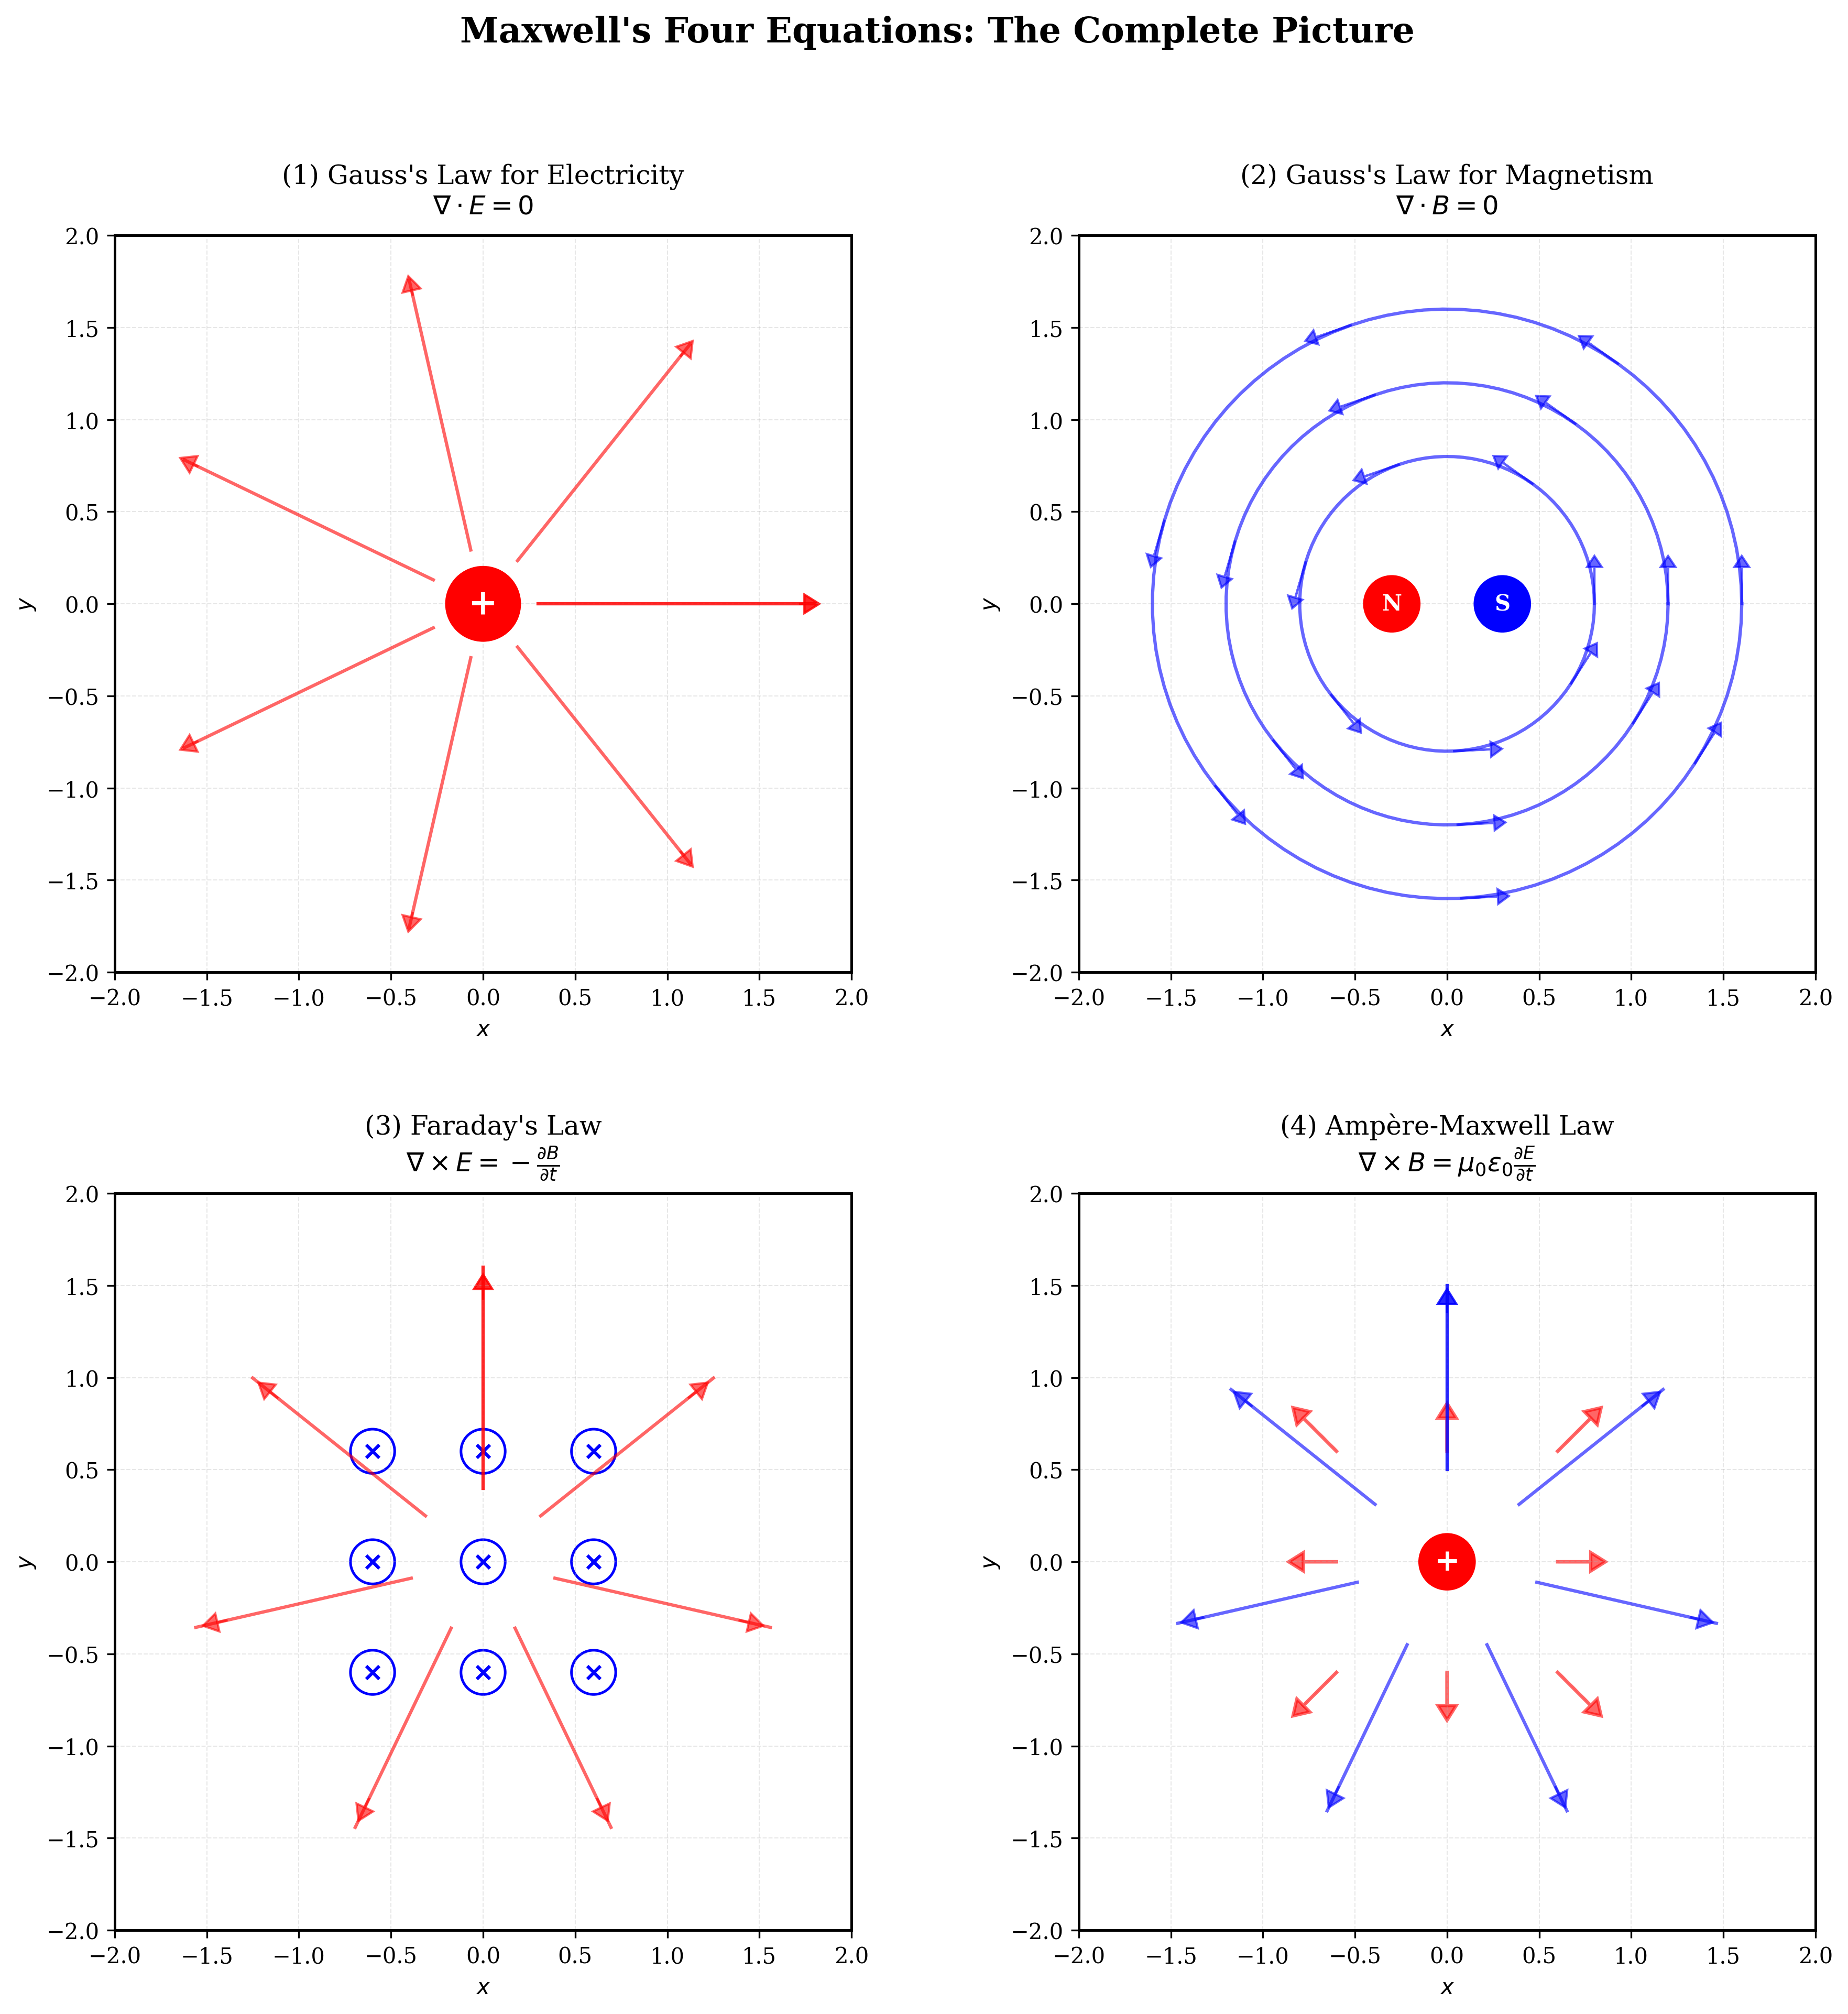
\includegraphics[width=0.9\textwidth]{images/chapter03/maxwell_equations_complete.png}
\caption{Visualization of all four Maxwell's equations. Top-left: Gauss's law for electricity shows electric field lines emanating from charges. Top-right: Gauss's law for magnetism shows closed magnetic field loops (no magnetic monopoles). Bottom-left: Faraday's law shows how changing magnetic fields create circulating electric fields. Bottom-right: Ampère-Maxwell law shows how changing electric fields create circulating magnetic fields.}
\label{fig:maxwell_complete}
\end{figure}

\subsection{The Vector Operators}

To understand these equations, we need the vector differential operators:

\begin{itemize}
    \item \textbf{Divergence} ($\nabla \cdot$): Measures how much a vector field spreads out from a point. For a vector field $\boldsymbol{F} = (F_x, F_y, F_z)$:
    \begin{equation}
    \nabla \cdot \boldsymbol{F} = \frac{\partial F_x}{\partial x} + \frac{\partial F_y}{\partial y} + \frac{\partial F_z}{\partial z}
    \end{equation}
    Positive divergence indicates a source (field lines emerging), while negative divergence indicates a sink (field lines converging).
    
    \item \textbf{Curl} ($\nabla \times$): Measures the rotation or circulation of a vector field:
    \begin{equation}
    \nabla \times \boldsymbol{F} = \left( \frac{\partial F_z}{\partial y} - \frac{\partial F_y}{\partial z}, \frac{\partial F_z}{\partial x} - \frac{\partial F_x}{\partial z}, \frac{\partial F_y}{\partial x} - \frac{\partial F_x}{\partial y} \right)
    \end{equation}
    Non-zero curl indicates rotational motion in the field.
    
    \item \textbf{Laplacian} ($\Delta$ or $\nabla^2$): The divergence of the gradient, appearing in the wave equation:
    \begin{equation}
    \Delta = \nabla^2 = \frac{\partial^2}{\partial x^2} + \frac{\partial^2}{\partial y^2} + \frac{\partial^2}{\partial z^2}
    \end{equation}
\end{itemize}

\begin{figure}[htbp]
\centering
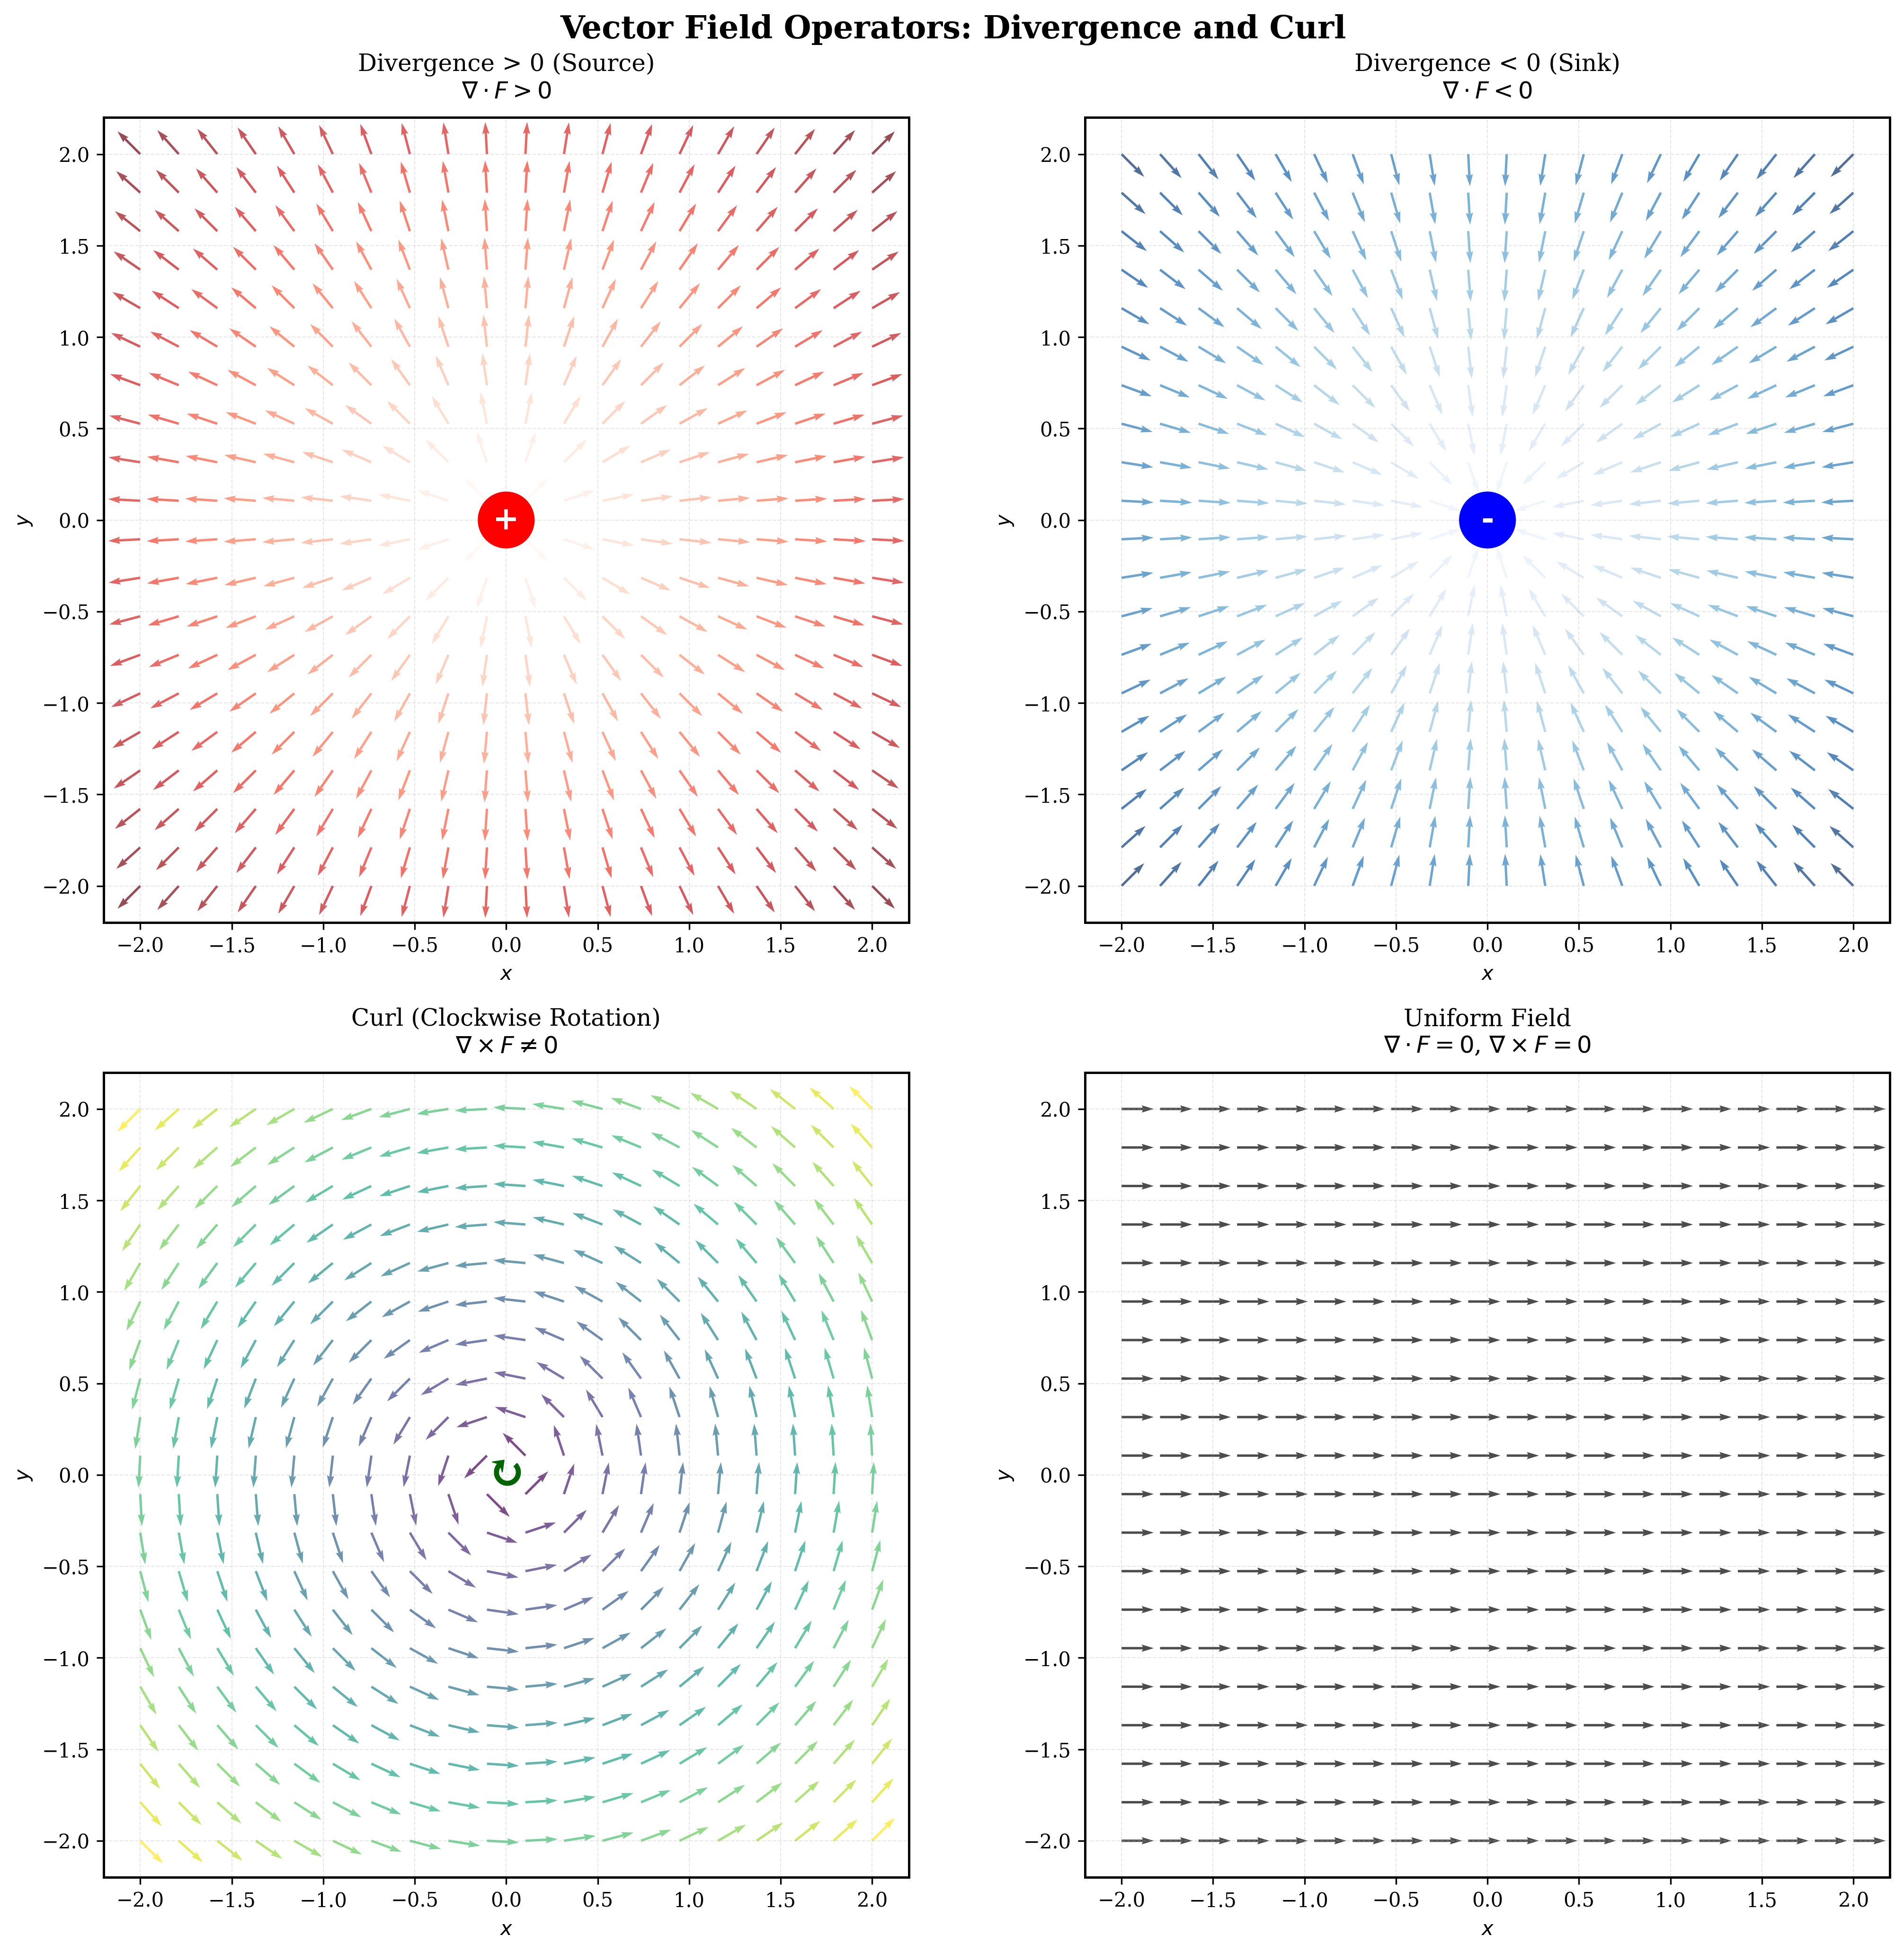
\includegraphics[width=0.9\textwidth]{images/chapter03/field_operators.png}
\caption{Visualization of vector field operators. Top-left: Positive divergence (source field) where field lines spread outward. Top-right: Negative divergence (sink field) where field lines converge. Bottom-left: Non-zero curl showing rotational motion. Bottom-right: Uniform field with zero divergence and curl.}
\label{fig:field_operators}
\end{figure}

\subsection{Light as an Electromagnetic Wave}

The profound insight from Maxwell's equations is that electric and magnetic fields can sustain each other in the absence of charges or currents, propagating through space as waves. When an electric field changes, it creates a changing magnetic field (via equation \eqref{eq:maxwell4-final}), which in turn creates a changing electric field (via equation \eqref{eq:maxwell2-final}), and so on. This self-sustaining oscillation propagates through space as an electromagnetic wave.

The speed of these waves, calculated from Maxwell's equations, is:
\begin{equation}
c = \frac{1}{\sqrt{\mu_0 \epsilon_0}} \approx 3 \times 10^8 \,\text{m/s}
\end{equation}

This value exactly matches the measured speed of light, leading Maxwell to conclude that light itself is an electromagnetic wave. This unification of optics and electromagnetism was one of the greatest achievements of 19th-century physics.

\subsection{The Wave Nature of Light}

The wave equation that emerges from Maxwell's equations (derived in the next section) has solutions of the form:
\begin{equation}
\boldsymbol{E}(\boldsymbol{r}, t) = \boldsymbol{E}_0 \cos(\omega t - \boldsymbol{k} \cdot \boldsymbol{r})
\end{equation}

where $\boldsymbol{E}_0$ is the amplitude vector, $\omega = 2\pi f$ is the angular frequency, $\boldsymbol{k}$ is the wave vector (pointing in the direction of propagation with magnitude $|\boldsymbol{k}| = 2\pi/\lambda$), and $\boldsymbol{r}$ is the position vector.

This solution describes a wave propagating through space with:
\begin{itemize}
    \item \textbf{Frequency} $f$: The number of oscillations per second
    \item \textbf{Wavelength} $\lambda$: The distance over which the wave repeats
    \item \textbf{Amplitude} $|\boldsymbol{E}_0|$: The maximum strength of the electric field
    \item \textbf{Energy}: Proportional to the square of the amplitude, $E \propto |\boldsymbol{E}_0|^2$
    \item \textbf{Intensity}: Also proportional to $|\boldsymbol{E}_0|^2$, representing the energy per unit area per unit time
\end{itemize}

The classical wave theory of light successfully explained many phenomena, including interference patterns in the double-slit experiment (first performed by Thomas Young in 1802), diffraction, and polarization. However, as we shall see in subsequent sections, certain experimental observations—particularly the photoelectric effect—could not be explained by this purely wave-based description, ultimately leading to the development of quantum mechanics.

\section{Wave Equation Derivation}
% 3.2 Wave Equation Derivation
% - From Maxwell's equations to wave equation
% - Solution: E(r,t) = E_0 Re{e^(i(ωt - k·r))}
% - Energy and intensity

\section{The Photoelectric Effect}
% 3.3 The Photoelectric Effect
% - Experimental observations
% - Einstein's explanation
% - Energy quantization: E_photon = hf = ℏω
% - Equation: eU = hf - W_0

\section{Wave-Particle Dualism}
% 3.4 Wave-Particle Dualism
% - Light as both wave and particle
% - De Broglie hypothesis for matter
% - De Broglie wavelength: λ = h/p = h/(mv)
% - Examples and implications

\section{The Need for Quantum Mechanics}
% 3.5 The Need for Quantum Mechanics
% - Limitations of classical physics
% - Experimental evidence summary
% - Transition to quantum theory
